% Basic stuff
\documentclass[a4paper,10pt]{article}
\usepackage[swissgerman]{babel}

% 3 column landscape layout with fewer margins
\usepackage[landscape, left=0.5cm, top=0.75cm, right=0.75cm, bottom=1cm, footskip=15pt]{geometry}
\usepackage{flowfram}
\ffvadjustfalse
\setlength{\columnsep}{0.75cm}
\Ncolumn{3}

% Remove paragraph indentation
\setlength{\parindent}{0pt}

% For defining line spacing
\usepackage{setspace}

\usepackage{multicol}

% For inserting figures
\usepackage{wrapfig}

% For enumeration with letters
\usepackage[shortlabels]{enumitem}

% Define nice looking boxes
\usepackage[many]{tcolorbox}

% Base style for boxes
\tcbset{
  base/.style={
    boxrule=0.2mm,
    left=1.75mm,
    arc=0mm,
    fonttitle=\bfseries,
    colbacktitle=black!10!white,
    coltitle=black,
    toptitle=0.75mm,
    bottomtitle=0.25mm,
    title={#1}
  }
}
\definecolor{backcol}{RGB}{240,240,240}
\definecolor{brandblue}{rgb}{0, 0, 0}
\newtcolorbox{mainbox}[1]{
  colframe=brandblue,
  colback=backcol,
  base={#1}
}

\definecolor{backcol2}{RGB}{255,255,255}
\definecolor{brandblue2}{rgb}{0, 0, 0}
\newtcolorbox{subbox}[1]{
  colframe=black!20!white,
  colframe=brandblue2,
  colback=backcol2,
  base={#1}
}

\newtcolorbox{subbox_noTitle}[1][]{
  colframe=black!20!white,
  colframe=brandblue2,
  colback=backcol2,
  base={#1},
  title=#1
}


% Mathematical typesetting & symbols
\usepackage{amsthm, mathtools, amssymb, amsmath}
\usepackage{marvosym, wasysym}
\allowdisplaybreaks

% Algorithms
\usepackage{algorithm}
\usepackage{algpseudocode}
% Reduce space before and after algorithm
\usepackage{etoolbox}
\BeforeBeginEnvironment{algorithm}{\vspace{-1em}}
\AfterEndEnvironment{algorithm}{\vspace{-1em}}

% Tables
\usepackage{tabularx, multirow}
\usepackage{makecell}
\usepackage{booktabs}
\renewcommand*{\arraystretch}{2}

% Make enumerations more compact
\newenvironment{myitemize}
{\vspace{-0.25cm}\begin{itemize}}
{\end{itemize}}
\setlist[itemize]{leftmargin=10pt, itemsep=0.5pt}

\setlist[enumerate]{leftmargin=10pt, itemsep=0.75pt}

% To include sketches & PDFs
\usepackage{graphicx}

% For indicator function
\usepackage{dsfont}

% For hyperlinks
\usepackage{hyperref}
\hypersetup{
  colorlinks=true
}

% Metadata (fixing the inline title format)
\title{\textbf{Machine Learning in Finance and Insurance}}
\author{}
\date{}

% Reduces space above and below the title
\usepackage{titling}
\setlength{\droptitle}{-1.5cm}
% \posttitle{\par\vspace{-0.5cm}}

% Math helper stuff
\def\limn{\lim_{n\to \infty}}
\def\limxo{\lim_{x\to 0}}
\def\limxi{\lim_{x\to\infty}}
\def\limxn{\lim_{x\to-\infty}}
\def\sumk{\sum_{k=1}^\infty}
\def\sumn{\sum_{n=0}^\infty}
\def\R{\mathbb{R}}
\def\dx{\text{ d}x}
\def\P{\mathbb{P}}
\def\F{\mathcal{F}}
% \def\E{\mathcal{E}}
\DeclareMathOperator{\E}{\mathbb{E}}
\DeclareMathOperator{\Var}{Var}

% Use small subtitles
\newcommand{\subtitle}[1]{\vspace{0.25cm}\begin{normalsize}\textbf{\textcolor{gray!150}{\uppercase{#1}}}\end{normalsize}}

% == Define commands for exercises and solutions ==
\definecolor{solutionGray}{RGB}{90,90,90}
\definecolor{exerciseBlack}{RGB}{0,0,0}
\definecolor{highlightGray}{RGB}{220,220,220}
% Counter for exercises
\newcounter{exerciseCounter}
\setcounter{exerciseCounter}{0}
% Command for exercises
\newcommand{\exercise}[1]{%
    \vspace{1mm}
    \stepcounter{exerciseCounter}%
    \color{exerciseBlack}
    % \textbf{\colorbox{highlightGray}{Ex \theexerciseCounter}}: #1
    \textbf{\underline{Ex \theexerciseCounter:}} #1
}
% Command for solutions
\newcommand{\solution}[1]{%
    {\color{solutionGray} \textbf{Sol: } #1} % solution text in gray
}


\begin{document}

% Add title
\maketitle

% Reduce space
\vspace{-3cm}


\begin{center}
    \textbf{Ramon Kaspar, ETH Zürich (Fall 2024)}
\end{center}

\begin{small}

\section{Basic Notions of Statistical Learn.}

\begin{subbox}{Expected Loss (Expected Risk)}
\[
\E[\ell(f(X), Y)] = \int_{\mathcal{X} \times \mathcal{Y}} \ell(f(x), y) \rho(dx, dy).
\]
For a measurable \textit{loss function} \(\ell : \mathcal{Y} \times \mathcal{Y} \to \R^+\)
\end{subbox}
Goal: Find \(f\) that minimizes \(\E[\ell(f(X), Y)]\).

\begin{subbox}{Empirical Loss (Empirical Risk)}
    With training data $(X_i, Y_i)_{i=1}^m$: 
    \[
        \E[\ell(f(X), Y)] \approx \frac{1}{m} \sum_{i=1}^m \ell(f(X_i), Y_i).
    \]
\end{subbox}
\(\Rightarrow\) Empirical loss minimizer depends on hypothesis class \(\mathcal{H}\) and loss function \(\ell\). For square loss and constant functions, the minimizer is \(\bar{Y} = \frac{1}{m} \sum_{i=1}^{m} Y_i\). There's a \textit{Bias-Variance Tradeoff}; the best balance depends on the unknown distribution of \(Y\).

\subtitle{Pred. Prob.:} 
Find meas. func. \(f: \mathcal{X} \rightarrow \mathcal{Y}\), s.t. \(f(X) \approx Y\).

\subtitle{Hypothesis Class:} 
A \textit{hypothesis class} is a family \(\mathcal{H}\) of measurable functions \(f : \mathcal{X} \to \mathcal{Y}\), e.g. all affine functions.

\subtitle{Model Estimation:}
Find a numerical solution \(\hat{f}_m\) to:
\begin{footnotesize}  
\[
\min_{f \in \mathcal{H}} \frac{1}{m} \sum_{i=1}^m \ell(f(X_i), Y_i)
\]
\end{footnotesize}
\begin{myitemize}
    \item \textbf{Deterministic algorithm:} \(\hat{f}_m(\cdot) = \hat{\varphi}\left( \cdot , (X_i, Y_i)_{i=1}^m \right)\)
    \item \textbf{Stochastic algorithm} (e.g., random initialization): \(\hat{f}_m(\cdot) = \hat{\varphi}\left( \cdot , (X_i, Y_i)_{i=1}^m, V \right)\), where \(V\) indep. of \((X, Y)\) \& random.
\end{myitemize}
Define the average model \(\hat{f}_m^{\text{avg}}(x) := \E[\hat{f}_m(x)]\).

\subtitle{Relationships between $X$ and $Y$:}
\vspace{0.2cm}
\begin{myitemize}
    \item \textit{Deterministic dependence:} $Y = g(X)$
    \item \textit{Homoscedastic additive noise:} $Y = g(X) + \epsilon$, for $\epsilon$ independent of $X$ with $\E[\epsilon] = 0$
    \item \textit{Heteroscedastic additive noise:} $Y = g(X) + h(X)\epsilon$, for $\epsilon$ independent of $X$ with $\E[\epsilon] = 0$
    \item \textit{Non-additive noise:} $Y = g(X, \epsilon)$, for $\epsilon$ independent of $X$
    \item \textit{Model-free:} the form of the underlying model is not known, only iid observations $(X_i, Y_i)_{i=1}^m$ are available
\end{myitemize}


\subtitle{Regression Function:}
\(\bar{f}(x)\) minimizes \(w \mapsto \\ \int_{\mathcal{Y}} \ell(w, y) \rho_{Y|X}(dy | x)\) and is called the \textit{regression function}. \\ \(\E[\ell(\bar{f}(X), Y)]\) is the \textit{irreducible error}.

\textbf{\textit{Square Loss}} \(\bar{f}(X) = \E[Y | X]\), \(\E[\ell(\bar{f}(X), Y)] = \Var(Y) - \Var(\E[Y | X])\) 

\textbf{\textit{Pinball Loss}}
\( \ell_{\alpha}(u) = \left( \alpha - 1_{\{u < 0\}} \right) u \text{ for } u \in \R \), \(\bar{f}(X) = q_\alpha\) and \(\E[\ell(\bar{f}(X), Y)] = \E \left[ \ell_\alpha( Y - q_\alpha(X) ) \right ])\) 

\begin{subbox}{Bias-Variance Decomposition of Square Loss}
\begin{align}
E\left[ (\hat{f}_m(X) - Y)^2 \right] = 
\underbrace{ \E \left[ \left( \hat{f}_m^{\text{avg}}(X) - \bar{f}(X) \right)^2 \right]}_{\text{Bias}^2} + \notag  \\
 \underbrace{E\left[ \left( \hat{f}_m(X) - \hat{f}_m^{\text{avg}}(X) \right)^2 \right] }_{\text{Variance}} \notag 
 + \underbrace{E\left[ \left( \bar{f}(X) - Y \right)^2 \right]}_{\text{Irreducible Error}}. \notag
\end{align}
\end{subbox}

% Insert Image Bia-Variance Tradeoff
\begin{wrapfigure}{r}{0.5\columnwidth}
    \centering
    \vspace{-20pt}
    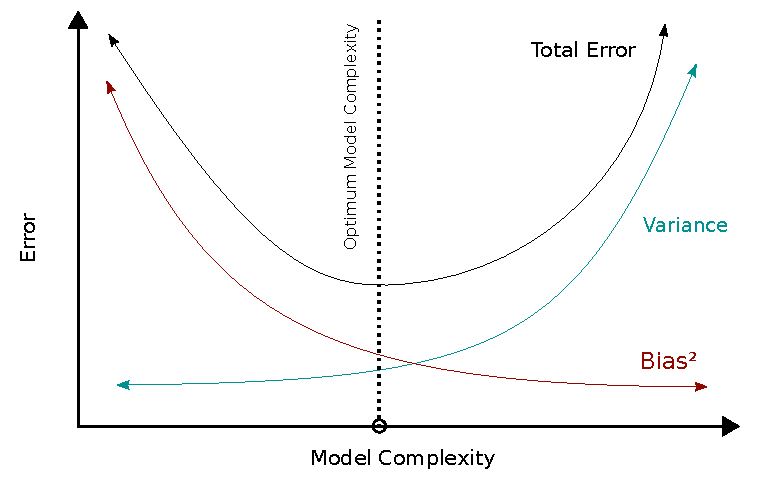
\includegraphics[width=0.45\columnwidth]{figures/Bias_and_variance_contributing_to_total_error.pdf}
    \vspace{-30pt}
\end{wrapfigure}

\textbf{Bias}: Error from erroneous assumptions (underfitting). \\
\textbf{Variance}: Error from sensitivity to data fluctuations (overfitting). \\
\textbf{Trade-off}: Increase model complexity $\Rightarrow$ lower bias, higher var

\begin{subbox}{$R^2$ \quad (goodness of in-sample fit)}
    Let $(X_i, Y_i)_{i=1}^m$ be the training data, and $(X_i, Y_i)_{i=m+1}^{m+n}$ the test data.
    Let $\hat{f}_m: \mathcal{X} \to \mathcal{Y}$ be a prediction function trained on training data:

    \[R^2 = 1 - \frac{SSR}{SST}\]

    $\text{SSR} = \sum_{i=1}^{m} \left( Y_i - \hat{f}_m(X_i) \right)^2$, $\text{SST} = \sum_{i=1}^{m} \left( Y_i - \overline{Y}_{\text{train}} \right)^2$ for $\quad \overline{Y}_{\text{train}} = \frac{1}{m} \sum_{i=1}^{m} Y_i$. \textit{The higher the better}.
\end{subbox}

Similarly, define out-of-sample \(R^2_{\text{os}}\) using test data; it measures \textbf{prediction power}.

\begin{subbox}{Approximation Error}
    $$\inf_{f \in \mathcal{H}} \mathbb{E} \, \ell(f(X), Y) - \mathbb{E} \, \ell(\overline{f}(X), Y) \geq 0$$
\end{subbox}
Approximation error occurs if $\mathcal{H}$ is not flexible enough to approximate $\bar{f}$ well. Is decreasing if $\mathcal{H}$ is increasing. Is $0$ if $\bar{f} \in \mathcal{H}$. 

If the empirical loss min. problem $\min_{f \in \mathcal{H}} \frac{1}{m} \sum_{i=1}^{m} \ell(f(X_i), Y_i)$ has a solution, we call it $\hat{f}_m^{\mathcal{H}} \in \mathcal{H}$.

\begin{subbox}{Sampling Error}
\begin{footnotesize}
    $$\E \left[ \ell \left( \hat{f}_m^{\mathcal{H}}(X), Y \right) \middle| \hat{f}_m^{\mathcal{H}} \right] 
- \inf_{f \in \mathcal{H}} \E [\ell(f(X), Y)] = $$
$$
\int_{\mathcal{X} \times \mathcal{Y}} \ell \left( \hat{f}_m^{\mathcal{H}}(x), y \right) \rho(dx, dy) 
- \inf_{f \in \mathcal{H}} \int_{\mathcal{X} \times \mathcal{Y}} \ell(f(x), y) \rho(dx, dy) \geq 0$$
\end{footnotesize}
\end{subbox}

Results from minimizing the empirical loss instead of the expected loss. Tends to decrease if the sample size $m$ is increasing.

\begin{subbox}{Direct Optimization Error}
Let $\hat{f}_m(\cdot) = \hat{\varphi}(\cdot, (X_i, Y_i)_{i=1}^{m}, V)
$:
    $$\frac{1}{m} \sum_{i=1}^{m} \ell \left( \hat{f}_m(X_i), Y_i \right) 
- \inf_{f \in \mathcal{H}} \frac{1}{m} \sum_{i=1}^{m} \ell \left( f(X_i), Y_i \right) \geq 0
$$
\end{subbox}
For classical methods (e.g., lin. reg.), assume \(\hat{f}_m \approx \hat{f}_m^{\mathcal{H}}\). For complex ML methods (boosted trees, NNs), typically \(\hat{f}_m \not\approx \hat{f}_m^{\mathcal{H}}\).

\begin{subbox}{Generalization Error}
\begin{footnotesize}
\[
\E\left[\ell(\hat{f}_m(X), Y) \mid \hat{f}_m\right]
= \E[\ell(\bar{f}(X), Y)] \quad \textit{(irreducible error)}
\]
\[
+ \inf_{f \in \mathcal{H}} \E[\ell(f(X), Y)] - \E[\ell(\bar{f}(X), Y)] \quad \textit{(approximation error)}
\]
\[
+ \E \left[\ell\left(\hat{f}_m^{\mathcal{H}}(X), Y\right) \mid \hat{f}_m^{\mathcal{H}}\right] - \inf_{f \in \mathcal{H}} \E[\ell(f(X), Y)] \quad \textit{(sampling error)}
\]
\[
+ \E \left[\ell\left(\hat{f}_m(X), Y\right) \mid \hat{f}_m\right] - \E \left[\ell\left(\hat{f}_m^{\mathcal{H}}(X), Y\right) \mid \hat{f}_m^{\mathcal{H}}\right] \textit{(ind. opt. error)}
\]
\end{footnotesize}
\end{subbox}
For fixed \(m \in \mathbb{N}\) and increasing \(\mathcal{H}\): approx. error decreases, sampling error increases (variance of \(\hat{f}_m^{\mathcal{H}}\) grows). There's a tradeoff between them (like bias-variance). For small data, \(\mathcal{H}\) should be simple; for large data, it can be complex.

\begin{subbox}{ Training Error and Test Error}
\begin{footnotesize}
$$E_{\text{tr}} = \frac{1}{m} \sum_{i=1}^{m} \ell\left(\hat{f}_m(X_i), Y_i\right), \ \ E_{\text{te}} = \frac{1}{m} \sum_{i=m+1}^{m+n} \ell\left(\hat{f}_m(X_i), Y_i\right)$$
\end{footnotesize}
\end{subbox}

If $E_{\text{tr}} \ll E_{\text{te}}$, the data most likely was overfitted. \\
\textbf{Sample Variance:} $\sigma_{\text{te}}^2 = \frac{1}{n-1} \sum_{i=m+1}^{m+n} \left( \ell\left(\hat{f}_m(X_i), Y_i\right) - E_{\text{te}} \right)^2$

\section{Linear Regression}

Linear regression models the relationship between predictors and response:
\(
y = \beta_0 + \beta_1 X_1 + \dots + \beta_d X_d + \epsilon, \quad \epsilon \sim N(0, \sigma^2)
\)
In matrix form:
\[
y = A\beta + \epsilon
\]
where \( A \) is the design matrix, \( \beta \) the coefficient vector.

\begin{subbox}{Normal Equation}
If $A^TA$ regular (or equivalently columns of $A$ lin. indep.):
\[
\hat{\beta} = \min_{b \in \mathbb{R}^{d+1}} \|A b - y\|_2^2
 = (A^\top A)^{-1} A^\top y
\]
\end{subbox}
$\Rightarrow \hat{\beta} = (A^T A)^{-1} A^T (A \beta + \epsilon) \sim \mathcal{N}_{d+1} \left( \beta, \sigma^2 (A^T A)^{-1} \right)$

If columns of \( A \) are linearly dependent, \( A^\top A \) is singular, and the normal equation has infinitely many solutions. The \textbf{pseudoinverse} solution \(\hat{\beta} = (A^\top A)^{\dagger} A^\top y\) minimizes \( \| b \|_2 \). Here, \((A^\top A)^{\dagger} = V \Lambda^{\dagger} V^\top\), with \(\Lambda^{\dagger}\) diagonal entries \(1_{\{\lambda_j > 0\}} \lambda_j^{-1}\).


\subtitle{Singular Value Decomposition (SVD)}

Matrix \( A \in \R^{m \times l}\), rank $r \leq \min(m,l)$, can be decomposed as:
\[
A = U \Sigma V^\top 
\]

\begin{myitemize}
    \item $U \in \R^{m \times m}$ and $V\in \R^{l \times l}$ orthogonal, $\Sigma^\dagger \in \R^{l \times m}$ diagonal
    \item $\lambda_1 \geq ... \geq \lambda_r$ are the positive eigenvalues of $A^\top A$ and $\Sigma = \text{diag}(\sqrt{\lambda_1}, ..., \sqrt{\lambda_r}, 0, ...) \in \R^{m \times l}$
    \item \textbf{Pseudoinverse} $A^\dagger = V \Sigma^\dagger U^\top$; for any $y \in \mathbb{R}^m, \hat{\beta} = A^{\dagger} y \in \mathbb{R}^n$ minimizes $b \mapsto \|A b - y\|_2$ with minimal $\|\cdot\|_2$-norm.
    \item \textbf{Regularization:} Truncate small \(\sigma_i\) (set \(\sigma_i = 0\) if \(\sigma_i < c\)); then \(\hat{\beta}_c = A_c^\dagger y \sim \mathcal{N}_l \left( Q_k \beta, \sigma^2 V \Lambda_c^{-1} V^T \right)\) balances bias and variance: increasing \( c \) increases bias and decreases variance.
\end{myitemize}

\begin{subbox}{Ridge Regression}
    $$\hat{\beta}_\lambda = \min_{b \in \mathbb{R}^{d+1}} \left( \|A b - y\|_2^2 + \lambda \|b\|_2^2 \right) = (A^\top A + \lambda I_l)^{-1} A^\top Y$$
\end{subbox}

\begin{footnotesize}
$\hat{\beta}_\lambda =  \sum_{i=1}^{r} \frac{\sigma_i}{\sigma_i^2 + \lambda} v_i u_i^T y \sim \mathcal{N}_l \left( \sum_{i=1}^{r} \frac{\lambda_i}{\lambda_i + \lambda} v_i v_i^T \beta, \sigma^2 \sum_{i=1}^{r} \frac{\lambda_i}{(\lambda_i + \lambda)^2} v_i v_i^T \right)$
\end{footnotesize}
\textit{Increasing \( \lambda \) increases bias and decreases variance}. 

\begin{subbox}{LASSO Regression}
\[
\hat{\beta}_\lambda = \min_{b \in \mathbb{R}^{d+1}} \left( \|A b - y\|_2^2 + \lambda \| \beta \|_1 \right)
\]
\end{subbox}
$\Rightarrow$ No closed-form solution, LASSO-Regr. encourages \textbf{sparsity}.

\subtitle{Cross-Validation}

Technique to estimate model's predictive performance and tune hyperparameters.
\begin{subbox_noTitle}
Divide data into \( K \) folds:
\begin{itemize}
    \item Train on \( K-1 \) folds.
    \item Validate on the remaining fold.
    \item Repeat \( K \) times; average validation error.
\end{itemize}
\end{subbox_noTitle}

\subtitle{Standardized Linear Regression} 
\[
\tilde{x}_i = \frac{x_i - \bar{x}}{s_x}, \quad  \tilde{y}_i = \frac{y_i - \bar{y}}{s_y}
\]
with mean \( \bar{x}_j \) and $s_j^2 = \frac{1}{m} \sum_{i=1}^{m} \left( x_{ij} - \bar{x}_j \right)^2$. The prediction $\hat{y}$ for a new datapoint $x=(x_1,...,x_d)$ is $\hat{y} = s_y \sum_{j=1}^{d} \frac{x_j - \bar{x}_j}{s_j} \hat{\beta}_j + \bar{y}$

\section{Gradient Descent}

A function $ h : \mathbb{R}^d \to \mathbb{R}$ is said to be \textbf{\textit{convex}} if $
h(\lambda x + (1 - \lambda) y) \leq \lambda h(x) + (1 - \lambda) h(y)$, for all $ x, y \in \mathbb{R}^d \text{ and } \lambda \in (0,1)$.

\textbf{Setup}: Given a convex function \( h: \mathbb{R}^d \to \mathbb{R} \) with minimizer \( x^* \), start at \( x_0 \) (might be random) and update with gradient steps:
\[
x_{k+1} = x_k - \eta_k \nabla h(x_k)
\]

If $\|\nabla h(x_k)\|_2 \leq L$  for all  $k$, then:
\[
\min_{0 \leq k \leq K} h(x_k) - h(x^*) \leq \frac{\|x_0 - x^*\|_2^2 + L^2 \sum_{k=0}^{K} \eta_k^2}{2 \sum_{k=0}^{K} \eta_k}
\]
If \( \sum_{k=0}^\infty \eta_k^2 < \infty \) and \( \sum_{k=0}^\infty \eta_k = \infty \), then \( h(x_k) \to h(x^*) \).

For accuracy $\varepsilon$, one needs $K = \left\lceil \left( \frac{L \| x_0 - x^* \|_2}{\varepsilon} \right)^2 \right\rceil$ gradient steps (which does not depend on the dimension!).

\begin{subbox}{Stochastic Gradient Descent (SGD)}
Consider $ H : \Omega \times \mathbb{R}^d \to \mathbb{R} $, convex in $ \theta $, measurable in $ \omega $, with $ \mathbb{E}[|H(\theta)|] < \infty $ for all $ \theta \in \mathbb{R}^d $. Let $ H_i $ be independent copies of $ H $, and $ I \in \mathbb{N} $. Define the gradient estimator:

$$
g_k(\theta) = \frac{1}{I} \sum_{i=kI+1}^{(k+1)I} \nabla H_i(\theta) \approx \nabla h(\theta), \quad k \geq 0.
$$

Start with $ \theta_0 \in \mathbb{R}^d $ (random) and perform updates:
$$
\theta_{k+1} = \theta_k - \eta_k \, g_k(\theta_k), \quad k \geq 0.
$$

For $ I = 1 $: SGD; for $ I > 1 $: SGD with mini-batches.

\end{subbox}

Let $\widetilde{H}_i$, $i = 1,\dots,v$, be independent copies of $H$, independent of $H_i$ (\textit{validation set}). Monitor the \textit{empirical loss} $\frac{1}{v} \sum_{i=1}^{v} \widetilde{H}_i(\theta_k)$ for $\theta_k$, $k = 0,1,\dots$. If the validation loss stops decreasing, decrease the learning rate $\eta_k$; if it increases, stop the SGD.

\section{Logistic Regression }

\begin{subbox}{Logistic Regression $\quad \quad$ (Binary Classification)}
    Let $Y \mid X \sim \text{Ber}(p(X))$, where $X = (X_1, \dots, X_d), p(X) = \psi\left(\beta_0 + \beta_1 X_1 + \dots + \beta_d X_d\right)$ and $\psi(x) = \frac{e^x}{e^x + 1} = \frac{1}{1 + e^{-x}}$.

    The empirical loss function, derived from conditional negative log-likelihood, corresponds to the \textit{cross-entropy loss}:
    
    \begin{align*}
    \hat{b} & = \min_{b \in \mathbb{R}^{d+1}} \sum_{i=1}^{m} \left\{ -y_i \log(\psi(x_i^T b)) - (1 - y_i) \log(1 - \psi(x_i^T b)) \right\} \\ 
    & = \min_{b \in \mathbb{R}^{d+1}} \sum_{i=1}^{m} \left\{ \log(1 + e^{x_i^T b}) - y_i x_i^T b  \begingroup \color{gray} \underbrace{ + \lambda ||b||_2}_{\text{Regularization}}  \endgroup \right \}
    \end{align*}

\end{subbox}

$\Rightarrow$\textit{Convex} min. problem in $b \in \R^{d+1}$, can be solved with (S)GD. \\

Having obtained $\hat{\beta} = (\hat{\beta}_0, \dots, \hat{\beta}_d)$ from the empirical loss minimization, we predict $Y = 1$ for a new data point $X = (x_1, \dots, x_d)$ by computing:
$
\hat{p}(x) = \psi\left( \hat{\beta}_0 + \sum_{j=1}^{d} x_j \hat{\beta}_j \right).
$
Using a decision \\ threshold $c \in (0, 1)$, we predict:
$
\hat{y}(x) = \begin{cases}
1, & \text{if } \hat{p}(x) \geq c, \\
0, & \text{if } \hat{p}(x) < c.
\end{cases}
$


% Having the solution of the empirical loss minimization problem: $\hat{\beta} = (\hat{\beta}_0, . . . , \hat{\beta}_d)$, we can predict the probability $Y=1$ conditioned on a new datapoint $X = (x_1, ..., x_d)$ by $\hat{p}(x) = \psi \left( \hat{\beta}_0 + \sum_{j=1}^{d} x_j \hat{\beta}_j \right)$. We then choose a \textit{decision threshold} $c \in (0, 1)$ and predict $Y$ to be $\hat{y}(x) = 1$ if $\hat{p}(x) \geq c$ and $\hat{y}(x) = 0$ if $\hat{p}(x) < c$.

\subtitle{Performance Metrics (Diagnostics)}  
\vspace{-0.2cm} % More compact
\begin{align*}
\text{TPR (Recall)}&=\frac{TP}{P} \quad &  \text{FPR}&=\frac{FP}{N} \quad & \text{FDR}&=\frac{FP}{TP+FP}
\end{align*}
\begin{align*}
\text{Accuracy}&=\frac{TP + TN}{P+N} \quad \quad    &  \text{Precision (PPV)}&=\frac{TP}{TP+FP}            
\end{align*}
$$
\text{F1 Score} = 2 \frac{\text{TPR} \times \text{PPV}}{\text{TPR} + \text{PPV}} = \frac{2 \text{TP}}{2 \text{TP} + \text{FP} + \text{FN}} = \frac{2}{\frac{1}{\text{Precision}} + \frac{1}{\text{Recall}}}
$$

\textbf{ROC}: plots TPR vs. FPR for $c \in [0, 1]$. Random guessing produces the diagonal with $AUC = 1/2$.
\textbf{AUROC} (Area under ROC): the larger the better (1 indicates a perfect classifier).

\subtitle{Credit Analytics}

Let $P$ be a good borrower and $N$ a bad borrower.

Try to \textit{minimize} $\text{FDR} = FP/(FP + TP)$ (FP’s result in losses), Try to \textit{maximize} $\text{TPR} = TP/P$ (increases business volume). 

$\Rightarrow$ Try to obtain a flat FDR/TPR-curve, i.e., a small area under the plotted FDR/TPR-curve is desirable.


\section{Support Vector Machine (SVM)}

\textbf{Derivation (Hard-margin SVM):} 
Let $ (x_i, y_i) \in \mathbb{R}^d \times \{-1, 1\} $ for $ i = 1, \dots, m $, with linear classification, i.e., there exist $ w \in \mathbb{R}^d $ and $ b \in \mathbb{R} $ such that
$
\operatorname{sign}(\langle w, x_i \rangle + b) = y_i \text{ for all } i.
$
Each classifier $ (w, b) $ defines the decision hyperplane:
$
H(w, b) = \{ x \in \mathbb{R}^d : \langle w, x \rangle + b = 0 \}.
$
The distance from $ x_i $ to $ H(w, b) $ is:
$
d_i = \frac{|\langle w, x_i \rangle + b|}{\|w\|},
$
and the margin is the minimal distance:
$
\gamma = \min_{i} d_i.
$
We aim to maximize the margin:
$
\max_{w, b} \gamma
$
subject to:
$
y_i (\langle w, x_i \rangle + b) \geq \gamma \|w\| \quad \forall i.
$
By scaling $ w $ and $ b $ such that $ \gamma \|w\| = 1 $, the constraints simplify to:
$
y_i (\langle w, x_i \rangle + b) \geq 1,  \forall i.
$
Maximizing $ \gamma $ is equivalent to minimizing $ \|w\| $, yielding:

\begin{subbox}{Hard-margin SVM}
$$
\min_{w, b} \|w\|^2
\quad 
\text{s.t. }
y_i (\langle w, x_i \rangle + b) \geq 1 \quad  \forall i \in \{1, \dots, m\}.
$$
\end{subbox}

\textbf{Problem:} Linear separation may be infeasible or lead to overfitting. Solutions using \textit{RKHS learning}:

\begin{myitemize}
    \item Lift $x_i$ into a \textit{Hilbert space} $H_0$ via a feature map $\Phi : \mathbb{R}^d \to H_0$. The classifier becomes $w \in H_0$.
    \item Introduce \textit{slack variables} $\xi_i \geq 0$ to allow constraint violations with a penalty in the objective.
\end{myitemize}

\begin{subbox}{Soft-margin SVM (Kernelized)}
    \begin{footnotesize}
    \begin{align*}
        \hat{w}_{SVM} &=
    \min_{w,b,\xi} 
    \| w \|_2^2 + C \sum_{i=1}^{m} \xi_i  \quad 
    \text{s.t. }  \ y_i \left( \left\langle w, \Phi(x_i) \right\rangle + b \right) \geq 1 - \xi_i \\
    &= \min_{(w,b) \in H_0 \times \R} 
    \| w \|_2^2 + \lambda \sum_{i=1}^{m} \underbrace{\max \left( 0, 1-  y_i ( \left\langle w, \Phi(x_i) \right\rangle + b \right ) )}_{\text{Hinge loss}} \\
    &= \min_{f \in H} \frac{1}{m} \sum_{i=1}^{m} \ell_{\text{Hinge}}(y_i, f(x_i)) + \lambda \|f\|_H^2 \\
    & 
    {\scriptstyle
    \quad \quad \text{where } H = \{f : \R^d \to \R : f = \langle w, \Phi(\cdot) \rangle \} \text{ is a Hilbert Space}}
    \end{align*}
    \end{footnotesize}
\end{subbox}

\textbf{Support Vector Regression (SVR)}:
Find $ (w, b) \in H_0 \times \mathbb{R} $ to approximate $ y \in \mathbb{R} $. Goal: Fit data within an $ \epsilon $-tube around $ f(x) = \langle w, \Phi(x) \rangle + b $.
The optimization problem becomes: \\
$ 
\min_{(w,b,\xi)} \|w\|^2 + C \sum_{i=1}^{m} \xi_i
$
s.t. $ |y_i - \langle w, \Phi(x_i) \rangle - b| \leq \epsilon + \xi_i$ with $\xi_i \geq 0 $.
Or similarly:
$
\min_{f \in H} \lambda \|f\|_H^2 + \frac{1}{m} \sum_{i=1}^{m} \ell_{\epsilon}(y_i, f(x_i)+b) 
$
where $ \epsilon $-insensitive loss $ \ell_\epsilon(y, y') = \max(0, |y - y'| - \epsilon) $.

\newpage

\section{Kernels \& Hilbert Spaces}

\begin{subbox_noTitle}
    A function $k : \mathcal{X} \times \mathcal{X} \to \mathbb{R}$ is called a \textbf{kernel} on $\mathcal{X}$ if there exists a Hilbert space $H$ and a map $\Phi : \mathcal{X} \to H$ such that for all $x, x' \in \mathcal{X}$ we have $k(x, x') = \langle \Phi(x), \Phi(x') \rangle_H$.
\end{subbox_noTitle}

A function $k : \mathcal{X} \times \mathcal{X} \to \mathbb{R}$ is a \textbf{kernel} if and only if it is \textbf{symmetric} and \textbf{pos. semidefinite} ($ \sum_{i=1}^{n} \sum_{j=1}^{n} \alpha_i \alpha_j k(x_j, x_i) \geq 0$).

\begin{myitemize}
    \item Linear kernel: $k(x, x') = \langle x, x' \rangle$
    \item Polynomial kernel: $p \in \mathbb{N}$ and $c \in \mathbb{R}_+$, $k(x, x') = (\langle x, x' \rangle + c)^p$
    \item Gaussian kernel: for $\gamma > 0$, $k(x, x') = \exp\left(-\frac{\|x - x'\|_2^2}{\gamma^2}\right)$
    \item Compactly supported radial basis kernel: for $p > d/2$, $k(x, x') = \max\{1 - \|x - x'\|_2, 0\}^p$
    \item Radial basis function kernels: $k(x, x') = \phi(\|x - x'\|_2)$ for $\phi : \mathbb{R}_+ \to \mathbb{R}$. The factor $\gamma$, s.t. $k_\gamma(x, x') = \phi(\|x - x'\|_2/\gamma)$ is the \textit{bandwidth} (the higher, the smoother the function).
\end{myitemize} 

\textbf{Decomposition Rules:} 
$k(\mathbf{x}, \mathbf{y}) = k_1(\mathbf{x}, \mathbf{y}) + k_2(\mathbf{x}, \mathbf{y})$,
$k(\mathbf{x}, \mathbf{y}) = k_1(\mathbf{x}, \mathbf{y})k_2(\mathbf{x}, \mathbf{y})$,
$k(\mathbf{x}, \mathbf{y}) = f(\mathbf{x}) f(\mathbf{y})$,
$k(\mathbf{x}, \mathbf{y}) = c k(\mathbf{x}, \mathbf{y}) \text{ for } c > 0$,
$k(\mathbf{x}, \mathbf{y}) = k(\phi(\mathbf{x}), \phi(\mathbf{y}))$.

\subtitle{Reproducing kernel Hilbert spaces}

We call $H$ a \textbf{reproducing kernel Hilbert space (RKHS)}, if $\delta_x : H \to \mathbb{R}$ given by $\delta_x(f) := f(x)$ is continuous for all $x \in \mathcal{X}$. 

A kernel $k : \mathcal{X} \times \mathcal{X} \to \mathbb{R}$ is called a \textbf{reproducing kernel of $H$}, if $k(\cdot, x) \in H$ and $f(x) = \langle f, k(\cdot, x) \rangle$ for all $x \in \mathcal{X}, f \in H$. If such a kernel $k$ exists, we call $\Phi : \mathcal{X} \to H$ given by $\Phi(x) := k(\cdot, x)$ the canonical feature map.

\textbf{Theorem:} Every RKHS has a unique reproducing kernel, and conversely, every positive definite kernel $ k $ corresponds to a unique RKHS $ H $.

\begin{subbox}{Mercer's Theorem}
    If $k$ is a continuous, symmetric, positive definite kernel on a compact set $\mathcal{X}$, then:
    $
    k(x, x') = \sum_{i=1}^\infty \lambda_i \phi_i(x) \phi_i(x'),
    $
    where $\lambda_i \geq 0$ are eigenvalues and $\{\phi_i\}$ are orthonormal in $L^2(\mathcal{X})$. Furthermore, the RKHS $H$ associated with $k$ is:
    $
    H = \left\{ f = \sum_{i=1}^\infty a_i \phi_i : \sum_{i=1}^\infty \frac{a_i^2}{\lambda_i} < \infty \right\},
    $
    with inner product
    $
    \langle f, g \rangle_H = \sum_{i=1}^\infty \frac{a_i b_i}{\lambda_i},
    $
    for $f = \sum a_i \phi_i$, $g = \sum b_i \phi_i$.
\end{subbox}
% \textbf{Implications:} Mercer's Theorem provides the theoretical basis for expressing kernels as infinite-dimensional feature maps, allowing us to perform computations in an implicit high-dimensional space.

\begin{subbox}{Representer Theorem}
    Any minimizer $f \in H$ of the regularized empirical risk
    $
    \min_{f \in H} \lambda \|f\|_H^2 + \sum_{i=1}^{m} \ell(y_i, f(x_i))
    $
    admits a representation of the form
    $
    f^*(x) = \sum_{i=1}^{m} \alpha_i k(x_i, x)
    $
    for some coefficients $\alpha_i \in \mathbb{R}$.
\end{subbox}

\textbf{Implications:} Mercer's Theorem allows kernels to implicitly map data into high-dimensional spaces. Representer Theorem ensures solutions are finite sums over training data using kernels (\textit{kernel trick}).

\textbf{Corollary:} Let $\ell(y, y') = (y - y')^2$. Assume $x_1, \dots, x_m$ are distinct and $k$ is strictly positive definite. Then, the parameters $a = (\alpha_1, \alpha_2, \dots, \alpha_m)$ of the optimizer $f_m^* = \sum_{i=1}^{m} \alpha_i k(x_i, \cdot)$ from \textit{Representer Theorem} are given by

\[
a = (\lambda m I_m + K_m)^{-1} b,
\]

where $I_m \in \mathbb{R}^{m \times m}$ is the identity matrix, $K_m \in \mathbb{R}^{m \times m}$ is given by $K_m[i,j] = k(x_i, x_j)$, and $b = (y_1, \dots, y_m)$.

\subtitle{Numerical approaches}

\textbf{Regression:} $\hat{w} = \mathbf{\Phi}^\top \hat{\alpha}$ ( \texttt{sklearn.kernel\_ridge.KernelRidge}).
\textbf{Binary Classification:} Use SMO Algorithm. For \textit{Hinge loss} use \texttt{sklearn.svm.SVC}, for $\epsilon$-sens. loss use \texttt{sklearn.svm.SVR}. 

\vspace{0.1cm}
Analytic solution not feasible for large datasets. Solutions:

\begin{myitemize}
    \item \textbf{Feature selection}: select a subset $I \subset \{1,..., m\}, |I|= k < m$ and build an estimator of the form $\hat{f}(x) = \sum_{i \in I} \alpha_i k(x_i, x)$. E.g. Nyström (\texttt{sklearn.kernel\_approximation.Nystroem})
    \item\textbf{Preconditioning:} Approximate $A^{-1}$ via $BB^\top \approx A^{-1}$ to solve $Ax = b$ efficiently (e.g., FALKON).
\end{myitemize}

\subtitle{Function approximation with RKHS}

Kernel $k$ is \textbf{universal}, if for every continuous function $f : X \to R$ and $\epsilon > 0$, there exists $h \in H$ such that: $\|h -f \|_{\inf} \leq \epsilon$. 

\textbf{Examples:}  Exponential kernel: $k(x, x') = \exp(\gamma \langle x, x' \rangle) \text{ for } \gamma > 0$, 
Gaussian kernel: $k(x, x') = \exp\left(-\gamma \|x - x'\|_2^2\right) \text{ for } \gamma > 0$, 
Binomial kernel: $k(x, x') = (1 - \langle x, x' \rangle)^{-\alpha} \text{ for } \alpha > 0, \ \mathcal{X} \subseteq \{x \in \mathbb{R}^d : \|x\|_2 < 1\}$.


\textbf{Kernel Rate:} For estimators $ \hat{f}_m $ in RKHS with smoothness $ s $, the estimation error decreases at rate $ m^{-\frac{s}{2s + d}} $, i.e., \\
$
\lim_{m \to \infty} \mathbb{P} \left( \| \hat{f}_m^* - \bar{f} \|_2 \geq C m^{-\frac{s}{2s + d}} \right) = 0
$

\textbf{Minimax Rate:} This rate $ m^{-\frac{s}{2s + d}} $ is the optimal rate achievable by any estimator over functions with smoothness $ s $, i.e., 
$
\lim_{m \to \infty} \inf_{\hat{T}_m} \sup_{\theta \in \Theta} \mathbb{P} \left( \| \hat{T}_m - \bar{f}_\theta \|_2 \geq c m^{-\frac{s}{2s + d}} \right) = 1.
$

$\Rightarrow$ Kernel methods achieve optimal convergence rates for estimating $ \bar{f} $, making them effective for high-dimensional nonparametric regression. However, neural networks can be seen as kernel methods where the feature map is learned from data and thus better than any a-priori fixed kernel.

\clearpage

\section{Neural Networks}

\begin{subbox}{Definition Feedforward Neural Network (FNN)}
    A \textbf{FNN} is a function $F_{\theta}: \mathbb{R}^{N_0} \rightarrow \mathbb{R}^{N_L}$ defined as:
$$
F_{\theta} = F^{(L)} \circ \rho \odot F^{(L-1)} \circ \cdots \circ \rho \odot F^{(1)}
$$
\vspace{-0.5cm}
\begin{myitemize}
    \item each $F^{(k)}: \mathbb{R}^{N_{k-1}} \rightarrow \mathbb{R}^{N_k}$ an affine function: $ F^{(k)}(x) = W^{(k)} \cdot x + b^{(k)} $, where $W^{(k)} \in \mathbb{R}^{N_k \times N_{k-1}}$ are weights and $b^{(k)} \in \mathbb{R}^{N_k}$ biases,
    \item $N_k$ the number of neurons in the $k$-th layer and $(N_0, \dots, N_L) \in \mathbb{N}^{L+1}$ is the network's architecture,
    \item $\theta = ((W^{(k)}, b^{(k)}), k = 1, \dots, L)$ are network parameters,
    \item parameter space is $\mathbb{R}^{P(N_0,\dots,N_L)} \ni \theta$, with $P := P(N_0, \dots, N_L) = \sum_{k=1}^{L} N_k N_{k-1} + N_k$,
    \item $\rho: \mathbb{R} \rightarrow \mathbb{R}$ is the non-linear activation function applied to vectors element-wise.
\end{myitemize}
\end{subbox}

\begin{myitemize}
    \item $k = 0$ is the \textit{input layer}, $k = L$ is the \textit{output layer}, $k \in \{1, \dots, L-1\}$ are the \textit{hidden layers}. $L + 1$ is the \textit{number of layers} and $L$ is the \textit{depth},
    \item $\|N\|_{\infty} = \max_{0 \leq k \leq L} N_k$ is the \textit{width} of the network.
\end{myitemize}

\begin{algorithm}
\footnotesize
\caption{Forward propagation}
\begin{algorithmic}[1]
\Require Params $\theta = \left( \left(W^{(k)}, b^{(k)}\right), k = 1, \dots, L \right)$; datapoint $(x, y)$
\Ensure Loss value $\ell(F_{\theta}(x), y)$
\State $a^{(0)} := x$
\For{$k = 1, \dots, L - 1$}
    \State $\tilde{a}^{(k)} := W^{(k)} a^{(k-1)} + b^{(k)}$
    \State $a^{(k)} := \rho(\tilde{a}^{(k)})$
\EndFor
\State $\hat{y} := W^{(L)} a^{(L-1)} + b^{(L)}$
\State \Return $\ell(\hat{y}, y)$
\end{algorithmic}
\end{algorithm}

\begin{subbox}{Mini-batch Stochastic Gradient Descent (SGD)}
    \vspace{-0.3cm}
    $$
    \theta_0 \sim \mathbb{P}_{\text{initialization}}, \quad \theta_{t+1} = \theta_t - \eta_t \nabla_{\theta} \mathcal{L}(\theta, D_{t}) \big|_{\theta = \theta_t}
    $$
    where \( D_t \) is a mini-batch of size \( B \). For \( B = 1 \), this reduces to standard SGD.
\end{subbox}

\begin{myitemize}
    \item Non-convex loss $\Rightarrow$ SGD result depends on initialization.
    \item Identical initial weights (e.g., $\theta_0 = c$) lead to identical gradients $\Rightarrow$ Initialize weights differently.
\end{myitemize}

\textbf{\textit{Xavier Initialization}:} \ \ (often used in practice)
$$
W^{(k)}_{j,l} \sim \mathcal{N}\left(0, \frac{1}{N_k}\right), \quad b^{(k)} = 0,
$$
where $N_k$ is the width of the $k$-th layer.

\begin{algorithm}
\footnotesize
\caption{Back-propagation $\quad \mathcal{O}(L)$ time \& memory}
\begin{algorithmic}[1]
\Require Params $\theta = \left( \left(W^{(k)}, b^{(k)}\right), k = 1, \dots, L \right)$; datapoint $(x, y)$
\Ensure Gradient $\nabla_{\theta} \ell(F_{\theta}(x), y)$
\State Compute $\ell(F_{\theta}(x), y)$ using forward propagation
\State $\text{\texttt{grad}} \gets \nabla_{\hat{y}} \ell(\hat{y}, y)$
\State $\nabla_{W^{(L)}} \ell(\hat{y}, y) = \text{\texttt{grad}} \cdot {a^{(L-1)}}^{T}$
\State $\nabla_{b^{(L)}} \ell(\hat{y}, y) = \text{\texttt{grad}}$
\For{$k = L - 1, \dots, 1$}
    \State $\text{\texttt{grad}} \gets \nabla_{\tilde{a}^{(k)}} \ell(\hat{y}, y) = \text{\texttt{grad}}^{T} \cdot W^{(k+1)} \cdot \text{diag} \left( \rho'(\tilde{a}^{(k)}) \right)$
    \State $\nabla_{W^{(k)}} \ell(\hat{y}, y) = \text{\texttt{grad}} \cdot {a^{(k-1)}}^{T}$
    \State $\nabla_{b^{(k)}} \ell(\hat{y}, y) = \text{\texttt{grad}}$
\EndFor
\State \Return $\left( \left( \nabla_{W^{(k)}} \ell(\hat{y}, y), \nabla_{b^{(k)}} \ell(\hat{y}, y) \right) \text{ for } k = 1, \dots, L \right)$
\end{algorithmic}
\end{algorithm}

\newpage

\subtitle{Batch Normalization} \\
\textbf{Problem:} Parameter updates cause \textit{internal covariate shift}, slowing training. \\
\textbf{Solution:} Normalize activations in each layer using batch mean and variance:
$$
a_j^{(k)}(x_i) \leftarrow \frac{a_j^{(k)}(x_i) - \mu_j^{(k)}}{\sqrt{\sigma_j^{(k)2} + \epsilon}},
$$
\begin{footnotesize}
$$
\mu_j^{(k)} = \frac{1}{n_{\text{batch}}} \sum_{i=1}^{n_{\text{batch}}} a_j^{(k)}(x_i), \quad \sigma_j^{(k)2} = \frac{1}{n_{\text{batch}}} \sum_{i=1}^{n_{\text{batch}}} \left(a_j^{(k)}(x_i) - \mu_j^{(k)}\right)^2
$$
\end{footnotesize}
$\epsilon \approx 10^{-5}$ prevents division by zero, Gradients are backpropagated through normalization.

\subtitle{Regularization:} \\
Loss functions are typically regularized, i.e. minimize objective: 

$$
\tilde{\mathcal{L}}(\theta, D) = \mathcal{L}(\theta, D) + \lambda \mathcal{R}(\theta),
$$

\textbf{Ridge:} $\mathcal{R}(\theta) = \|\theta\|_2^2$ (shrinks $\theta$, prevents overfitting) \\
\textbf{Lasso:} $\mathcal{R}(\theta) = \|\theta\|_1$ (leads to sparse $\theta$) \\
\textbf{Notes:} Only weights $W$ are regularized (not biases), and different $\lambda$ can be used per layer.

\textbf{Training Techniques as Regularizers:}

\begin{myitemize}
    \item \textbf{Early Stopping:} Stop training if no improvement on validation set for $p$ steps (patience). Limits parameter space (similar to $L^2$-regularization).
    \item \textbf{Dropout:} Set each neuron to zero with probability $p$ before each gradient step; encourages sparse, redundant represent..
    \item \textbf{Other Techniques:} Bagging, dataset augmentation, weight robustness, parameter sharing.
\end{myitemize}

\subtitle{Neural Tangent Kernel (NTK)}

\textbf{Generalization Puzzle:} Overparametrized NNs generalize well despite classical bias-variance trade-off.

\textbf{Goal:} Study the dynamics of a NN $F_\theta : \R^{N_0} \to \R$ during GD.

\begin{subbox_noTitle}
For a NN \( F_{\theta} : \mathbb{R}^{N_0} \rightarrow \mathbb{R} \), the \textbf{NTK} is defined as:
\[
K(x, x'; \theta_t) = D_{\theta_t} F_{\theta}(x) \cdot D_{\theta} F_{\theta_t}(x')^\top \in \mathbb{R}.
\]
\end{subbox_noTitle}

Loss: $\mathcal{L}(\theta_t, D) = \frac{1}{m} \sum_{i=1}^m \ell(F_{\theta_t}(x_i), y_i)$.

Gradient flow: $\frac{d\theta_t}{dt} = - D_\theta \mathcal{L}(\theta_t, D)^\top$.

Using chain rule:
$\frac{d}{dt} \mathcal{L}(\theta_t, D) = - \frac{1}{m^2} \sum_{i,j=1}^m D_{\hat{y}} \ell(F_{\theta_t}(x_i), y_i) \cdot K(x_i, x_j; \theta_t) \cdot D_{\hat{y}} \ell(F_{\theta_t}(x_j), y_j)^\top 
= - \left\| D_{\hat{y}} \ell(F_{\theta_t}(\cdot), y) \right\|_{K(\cdot, \cdot, \theta_t), D}^2$


\subtitle{Convergence Results} [Jacot et. al, 2018]

\textbf{Theorem (NTK at Initialization):} For shallow NN $(N_0,N_1,1)$ with $\theta_0 \sim \mathcal{N}(0,I)$, as $N_1 \to \infty$:
$F_{\theta_0} \to \text{GP}(0,C)$ where
$C(x,x') = \mathbb{E}_{f \sim \text{GP}(0,\Sigma)}[\rho(f(x))\rho(f(x'))] + \beta^2$
with $\Sigma(x,x') = \frac{x^\top x'}{N_0} + \beta^2$

\textbf{Theorem (NTK During Training):} For any $T>0$ with bounded $\int_0^T \frac{1}{m}\sum_i \|D_{\hat{y}}\ell(F_{\theta_t}(x_i),y_i)\|_2^2dt$:
$\sup_{t\in[0,T]}\|K(x,x';\theta_t) - \tilde{K}(x,x')\| \xrightarrow{P} 0$ as width $\to \infty$.   

\subtitle{Minimum-Norm Solution}

For squared loss $\ell(\hat{y},y) = (\hat{y}-y)^2$, as $t \to \infty$:
$F_{\theta_\infty}(x) = F_{\theta_0}(x) + \sum_{i=1}^m \sum_{j=1}^m \tilde{K}^{(L)}(x,x_i)\bar{K}_{i,j}^{-1}(y_j - F_{\theta_0}(x_j))$
where $\bar{K}_{i,j} := \tilde{K}^{(L)}(x_i,x_j)$ (limiting NTK evaluated on dataset), First term is initial network output
and Second term is correction towards minimum-norm interpolator in RKHS.

\textbf{Key insight:} Solution converges to minimum-norm interpolator in NTK RKHS:
$\arg\min_{f \in \mathcal{H}, f(x_i)=y_i} \|f\|_{\mathcal{H}}$.

\subtitle{Generalization in Overparametrized Regime}

\textbf{Linear Regression Setting:}
Model: $Y = X^\top\beta + \epsilon$, $\epsilon \sim \mathcal{N}(0,\sigma^2)$, where $X=(X_1,...,X_p) \in \R^p$ with covariance $\Sigma$. $\rightarrow \hat{\beta} = (A^\top A)^\dagger A^\top Y$.

\textbf{Bias-Variance Decomposition} (conditioned on $A$): \vspace{-10pt}
$$\mathbb{E}[(\hat{f}_D(X) - f^*(X))^2|A] = \underbrace{\beta^\top\Pi\Sigma\Pi\beta}_{B_A=\text{bias}^2} + \underbrace{\frac{\sigma^2}{m}\text{Tr}(\hat{\Sigma}^\dagger\Sigma)}_{V_A=\text{variance}}$$
where $\hat{\Sigma} = \frac{1}{m}A^\top A$, $\Pi = I_p - \hat{\Sigma}^\dagger\hat{\Sigma}$

\textbf{Theorem (Asymptotic Variance):}
For $p,m\to\infty$ with $p/m\to\gamma$:
$V_A \to \sigma^2\frac{1-\max{1-\gamma,0}}{|1-\gamma|}$. \textit{[Hastie et al., 2022]}

\textbf{Double Descent Phenomenon:} $\gamma$ quantifies model complexity ($\gamma \gg 1 \Rightarrow p \gg m \Rightarrow $ Complex model). Variance increase for $\gamma \in (0,1)$ (classical bias-variance trade-off), but decreases for $\gamma > 1$ (overparametrized).


\begin{wrapfigure}{r}{0.5\columnwidth}
    \centering
    \vspace{-20pt}
    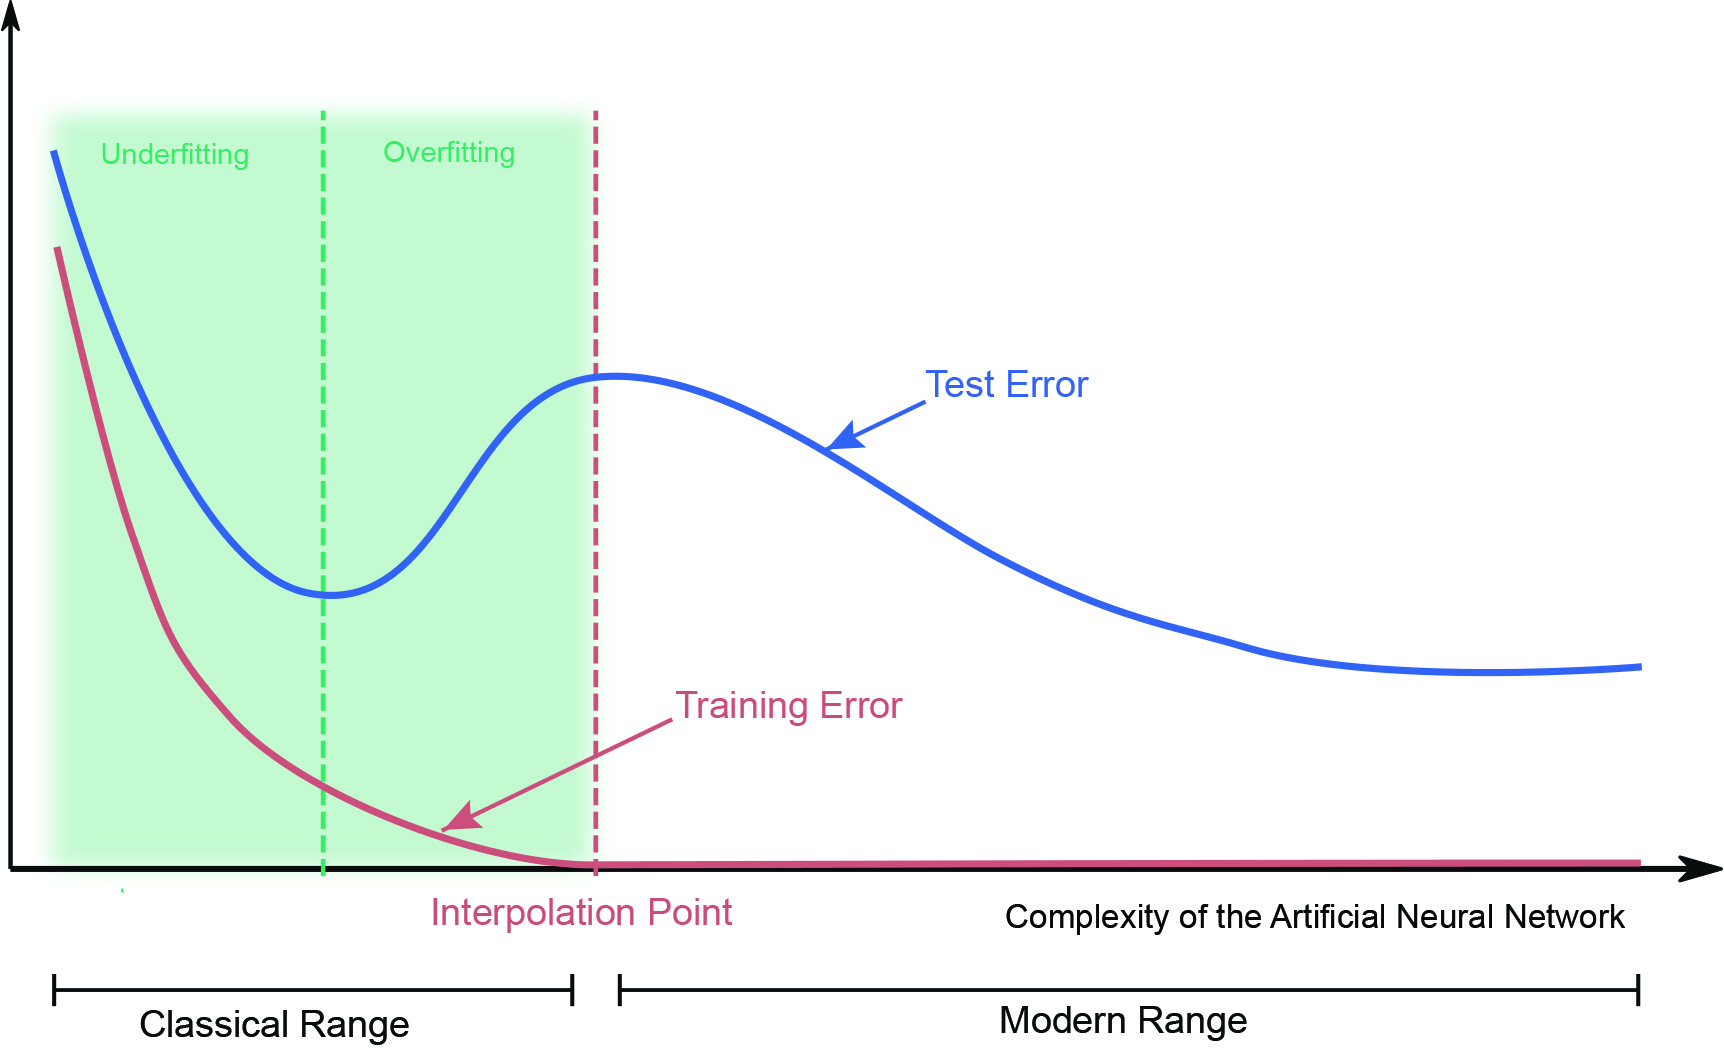
\includegraphics[width=0.45\columnwidth]{figures/double_descent_curve.jpg}
    \vspace{-30pt}
\end{wrapfigure}

$\Rightarrow$ Variance decreases as soon as model complexity passes the interpolation threshold. The test error can decrease even after the train error has reached zero.

\newpage

\section{Convolutional Neural Networks}

Three components: \textit{convolution-}, \textit{detector-} and \textit{pooling layer}.

\textbf{Convolutional layer:} Let $I \in \mathbb{R}^{n_1 \times n_2}$, $K \in \mathbb{R}^{m_1 \times m_2}$, $m_1 \leq n_1$, $m_2 \leq n_2$, then their \textbf{cross-correlation} ($I \circledast K$) is:
$$
(I \circledast K)_{i,j} := \sum_{m=1}^{m_1} \sum_{n=1}^{m_2} I_{m+i-1, n+j-1} K_{m, n}.
$$

\begin{myitemize}
    \item \textbf{Kernels:} Square $m \times m$ matrices ($m$ hyperparameter); convolution layer uses $M > 1$ kernels in parallel to produce multiple feature maps.
    \item \textbf{Padding ($p$):} 0's added around input to control output size.
    \item \textbf{Stride ($s$):} steps kernel moves over input matrix.
\end{myitemize}

Output size formula:$\left( \frac{n_1 + 2p - m}{s} + 1, \frac{n_2 + 2p - m}{s} + 1, M \right)$ \\

\textbf{Detector layer:}
Applies non-linear activation $\rho$ component-wise ($I_{i,j,k} \mapsto \rho(I_{i,j,k})$); output shape same as input; no trainable parameters.

\begin{wrapfigure}{r}{0.25\columnwidth}
    \centering
    \vspace{-25pt}
    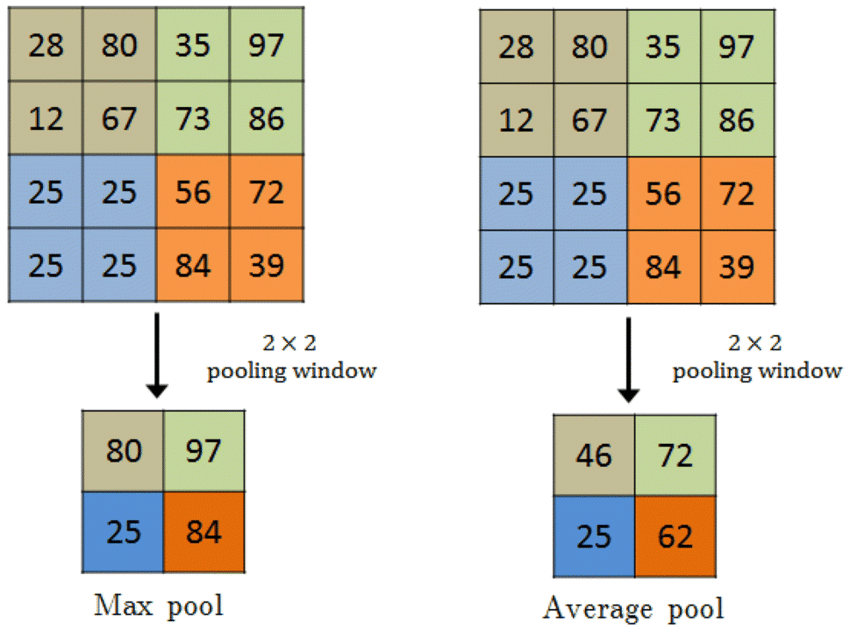
\includegraphics[width=0.27\columnwidth]{figures/Visual-representation-of-pooling-operations-a-max-pooling-b-average-pooling}
    \vspace{-20pt}
\end{wrapfigure}

\textbf{Pooling Layer:} Fixed filter (e.g., $m=2$, $s=2$, $p=0$); operates per channel; no trainable parameters.
\\

Convolution $\equiv$ Linear transformation via sparse, parameter-shared weights (doubly block-circulant matrix).

\begin{myitemize}
    \item \textbf{Parameter sharing:} Same kernel used at every position $\Rightarrow$ shared learning, translation equivariance.
    \item \textbf{Sparsity:} Small kernels reduce parameters $\Rightarrow$ computational efficiency; layers extract local (edges) to global (digits) features.
\end{myitemize}

\section{Recurrent Neural Networks}

\begin{wrapfigure}{r}{0.5\columnwidth}
    \centering
    \vspace{-25pt}
    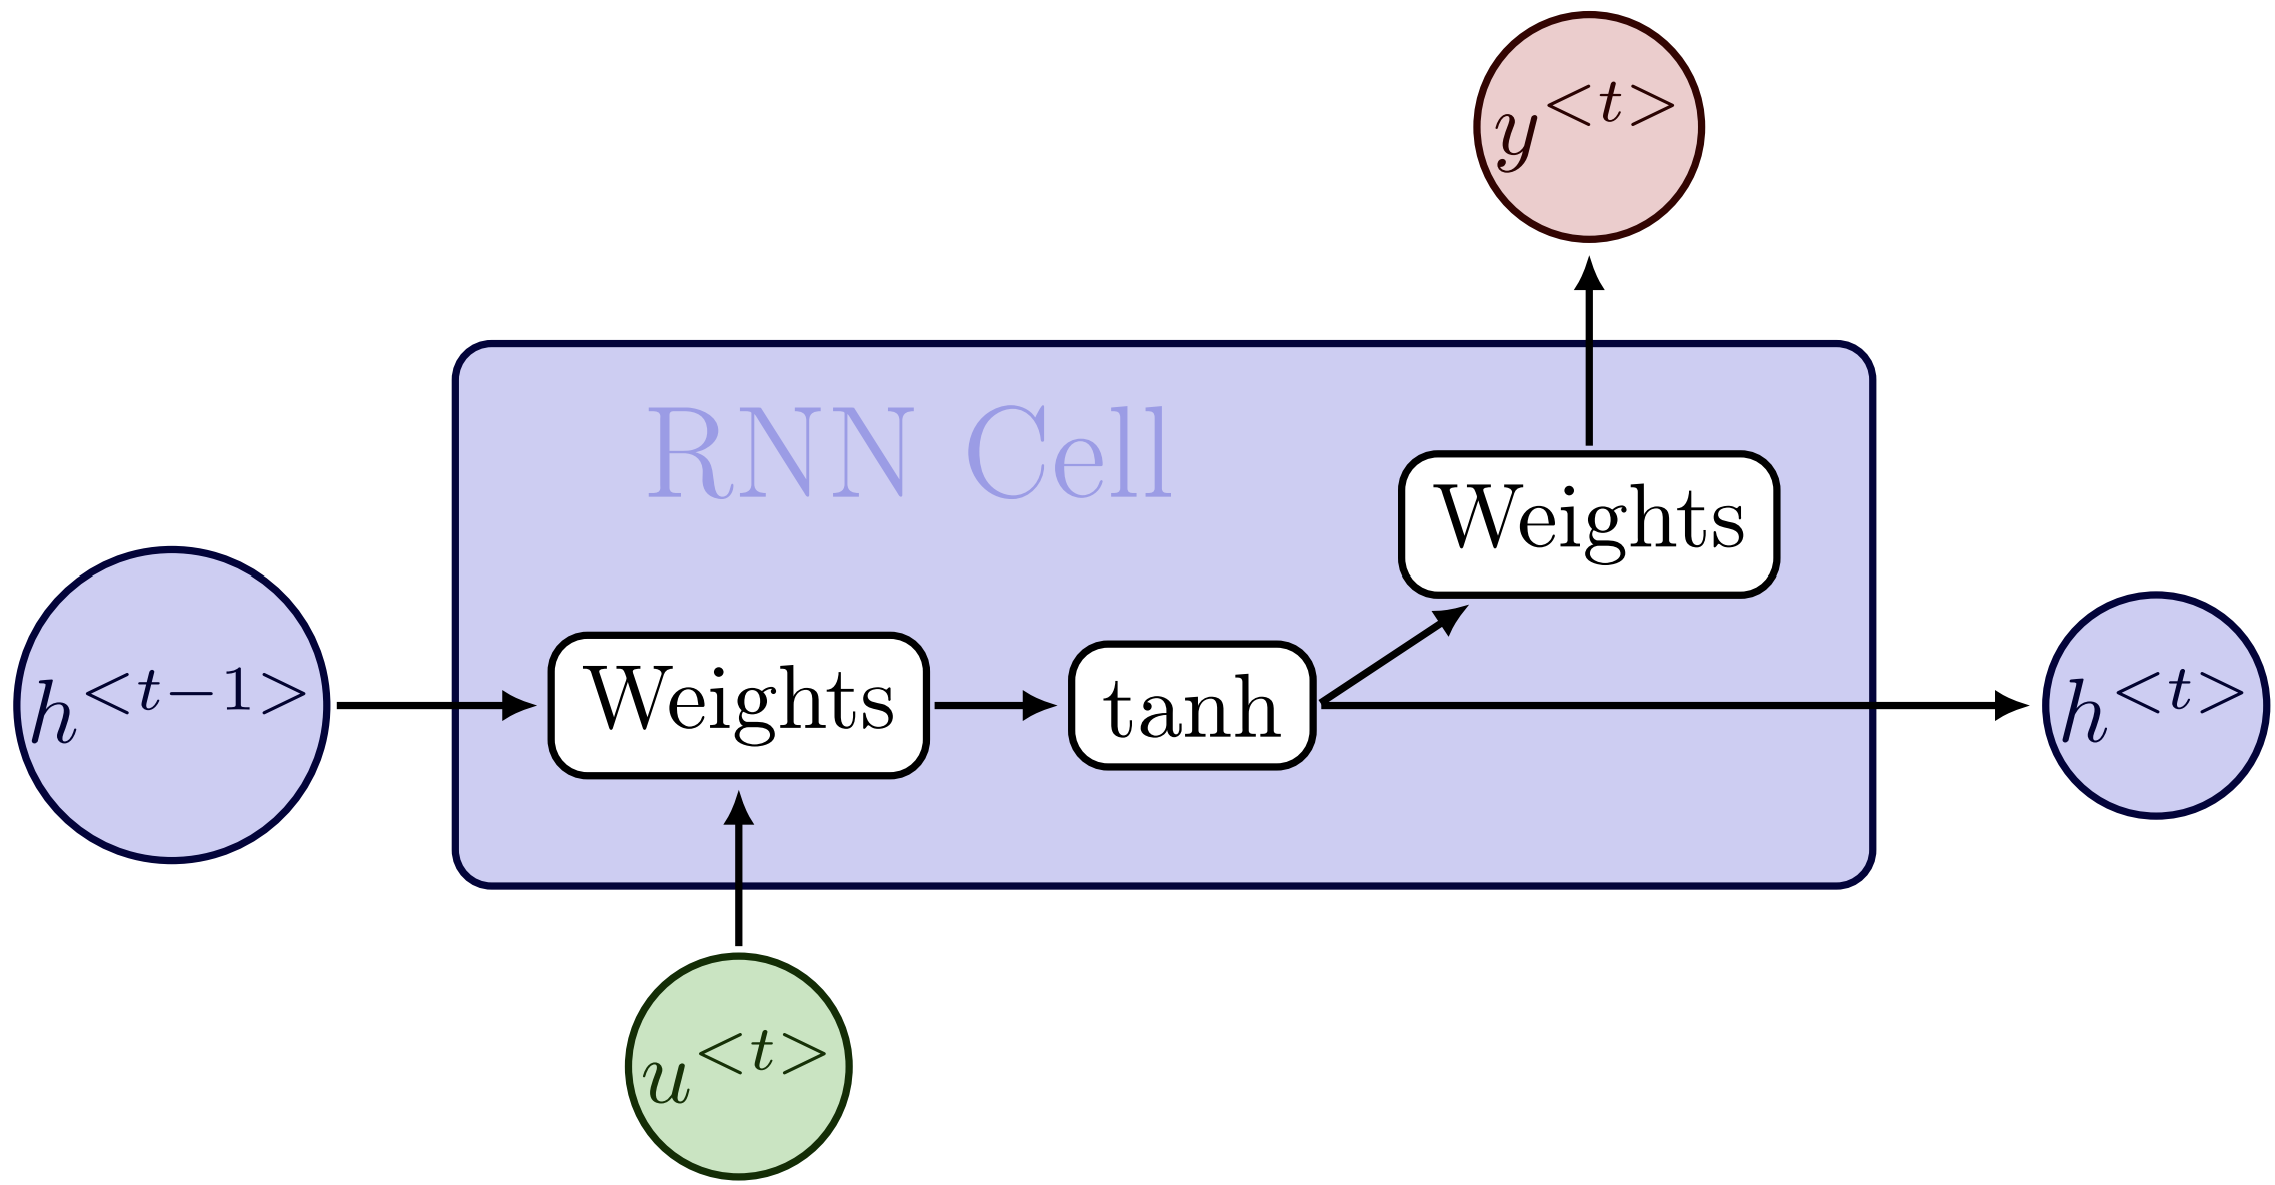
\includegraphics[width=0.5\columnwidth]{figures/RNN_cell.png}
    \vspace{-20pt}
\end{wrapfigure}

Exploit data priors of sequential data, $(x^{\langle 1 \rangle}, x^{\langle 2 \rangle}, \dots, x^{\langle T \rangle})$.

$$
\begin{cases}
a^{\langle t \rangle} = W \cdot h^{\langle t-1 \rangle} + U \cdot x^{\langle t \rangle} + b \\
h^{\langle t \rangle} = \rho(a^{\langle t \rangle}) \\
y^{\langle t \rangle} = V \cdot h^{\langle t \rangle} + c
\end{cases}
$$

Hidden states of RNN form a dynamical system with stationary
transition functions: $h^{\langle t \rangle} = f_{\theta}\left(h^{\langle t-1 \rangle}, x^{\langle t \rangle}\right)$. The parameter $\theta = (W, U, b)$ are used at each time step $t$ (\textbf{parameter sharing}). Hidden state $h^{\langle t \rangle}$ summarizes statistics of past sequence. \\

\textbf{Back-Propagation Through Time (BPTT):} Consider Loss $\mathcal{L} = \sum_{t=1}^{T} \mathcal{L}^{\langle t \rangle} = \sum_{t=1}^{T} \ell(\hat{y}^{\langle t \rangle}, y^{\langle t \rangle}), \quad t = 1, \dots, T$

Compute recursively the gradients of $\mathcal{L}$:
$
D_{\hat{y}^{\langle t \rangle}} \mathcal{L} = D_{\hat{y}^{\langle t \rangle}} \ell(\hat{y}^{\langle t \rangle}, y^{\langle t \rangle})
$ and
$
D_{h^{\langle t \rangle}} \mathcal{L} = D_{\hat{y}^{\langle t \rangle}} \mathcal{L} \cdot V + D_{h^{\langle t+1 \rangle}} \mathcal{L} \cdot \operatorname{diag}\left( \rho'\left(a^{\langle t+1 \rangle}\right) \right) \cdot W
$

\textbf{Vanishing/Exploding Gradient Problem:} Gradients increase/decrease exponentially over time steps:
$$
D_{\theta} \mathcal{L}^{\langle t \rangle} = \sum_{k=1}^{t} \left( \prod_{i=k+1}^{t} D_{h^{\langle i \rangle}} h^{\langle i+1 \rangle} \right) D_{h^{\langle k \rangle}} \mathcal{L}^{\langle t \rangle} \cdot D_{\theta} h^{\langle k \rangle}
$$
If $ \| D_{h^{\langle i \rangle}} h^{\langle i+1 \rangle} \| > 1 $, gradients \textit{explode}; if $ < 1 $, gradients \textit{vanish}.

\textbf{Solution to exploding gradient problem:} \textit{gradient clipping}; at each gradient step, if the gradient is larger than a threshold $K$, 'clip' it to $K$:

$$
D_\theta \mathcal{L} \leftarrow 
\begin{cases} 
D_\theta \mathcal{L} & \text{if } \|D_\theta \mathcal{L}\| < K \\ 
K \frac{D_\theta \mathcal{L}}{\|D_\theta \mathcal{L}\|} & \text{if } \|D_\theta \mathcal{L}\| \geq K 
\end{cases}
$$

\textbf{Solutions to vanishing gradient:}

\textbf{(1) GRU:} Two gates control information flow (by learning optimal gate parameters, model learns how to accumulate/forget past info dynamically):
$$\begin{cases}
\Gamma_r = \rho(W_r h^{\langle t-1 \rangle} + U_r x^{\langle t \rangle} + b_r)  \quad \quad \text{(reset)} \\
\Gamma_u = \rho(W_u h^{\langle t-1 \rangle} + U_u x^{\langle t \rangle} + b_u) \quad \quad \text{(update)} \\
h^{\langle t \rangle} = (1-\Gamma_u) \odot h^{\langle t-1 \rangle} + \Gamma_u \odot \tanh(W[\Gamma_r \odot h^{\langle t-1 \rangle}, x^{\langle t \rangle}])
\end{cases}$$

\textbf{(2) LSTM:} Memory cell $c^{\langle t \rangle}$ separates information flow:
$$\begin{cases}
\Gamma_f, \Gamma_i, \Gamma_o = \text{forget/input/output gates} \\
c^{\langle t \rangle} = \Gamma_f \odot c^{\langle t-1 \rangle} + \Gamma_i \odot \tilde{c}^{\langle t \rangle} & \text{(memory)} \\
h^{\langle t \rangle} = \Gamma_o \odot \tanh(c^{\langle t \rangle}) & \text{(output)}
\end{cases}$$


\section{Classification \& Regression Trees}

\textbf{Key Idea:} Transform input x into output y via sequence of simple binary decisions. \ \ \textbf{Advantages:}

\begin{itemize}
    \item Easy to interpret (medicine, insurance)
    \item Powerful with ensemble methods
    \item Can approximate any continuous function
\end{itemize}

\begin{subbox}{Binary Tree Definition}
    Triplet $(\mathcal{T}, \mathcal{P}, \mathcal{V})$ where:
    
\begin{myitemize}
    \item $\mathcal{T} \subseteq \bigcup_{l \in \mathbb{N}_0} \{0, 1\}^l$: nodes ($t^{\text{flip}}, t^{\text{cut}} \in \mathcal{T}$ if $t \in \mathcal{T} \setminus \{()\}$)
    \item $\mathcal{P} = \{P_t \subseteq \mathcal{X}\}$: partitions ($P_t \cup P_{t^{\text{flip}}} = P_{t^{\text{cut}}}$)
    \item $\mathcal{V} = \{y_t \in \mathcal{Y}\}$: values
\end{myitemize}
Tree function: $f(x) = \sum_{t \in \mathcal{T}} y_t \mathds{1}_{P_t}(x)$
\end{subbox} 

\begin{algorithm}[ht!]
\footnotesize
\caption{Basic structure of tree growing algorithm}
\begin{algorithmic}[1]
\State Initialize $\mathcal{T} = \{()\}$ and $P_{()} = \mathcal{X}$.
\While{Stopping criterion (*) is not reached}
    \State Choose a node $t \in \mathcal{T}$ ($t \in \{0, 1\}^l$), a variable $i \in \{1, \ldots, d\}$, and a set $C_i \subseteq \mathcal{X}_i$ according to criterion (**).
    \State Set $\mathcal{T} \leftarrow \mathcal{T} \cup \{t0, t1\}$, where $t0 = (t_1, t_2, \ldots, t_l, 0)$ and $t1 = (t_1, t_2, \ldots, t_l, 1)$.
    \State Set $P_{t0} = P_t \cap \{x \in \mathcal{X} : x_i \in C_i\}$, $P_{t1} = P_t \cap \{x \in \mathcal{X} : x_i \not\in C_i\}$.
\EndWhile
\State Compute the values $\mathcal{V} = \{y_t : t \in \mathcal{T}\}$; hereby, for all $t \in \mathcal{T}$, $y_t$ is calculated solely using the training data $\{y^i : i \in \{1, \ldots, m\}, x^i \in P_t\}$ according to criterion (***).
\State \Return $(\mathcal{T}, \mathcal{P}, \mathcal{V})$.
\end{algorithmic}
\end{algorithm}

\newpage
\subtitle{(***) How to assign values to leaves?}

\textbf{Node Statistics:} $p(t) = \frac{|\{i: x^i \in P_t\}|}{m}$, $p(y|t) = \frac{|\{i: x^i \in P_t, y^i = y\}|}{|\{i: x^i \in P_t\}|}$ Here, $p(t)$ is the estimated probability of an input $x$ belonging to the set $P_t$, and $p(y | t)$ the likelihood of $y$ being the output given that an input $x$ belongs to the set $P_t$. 

\textbf{Regression ($\mathcal{Y} \in \R$):} $y_t = \frac{1}{|\{i: x^i \in P_t\}|}\sum_{i: x^i \in P_t} y^i$ (emp. mean)

\textbf{Classification ($\mathcal{Y} = \{1,...,K \}$):} $y_t = \arg\max_{c \in \mathcal{Y}} |\{i: x^i \in P_t, y^i = c\}|$ (majority vote)

\textbf{General:} $y_t \in \arg\min_{y \in \mathcal{Y}} \sum_{i=1}^m L(y,y^i) \mathds{1}_{x^i \in P_t}$ (empirical mean for $L(y, y')=(y-y')^2$, majority vote for $L(y, y')=\mathds{1}_{y \neq y'}$.


\subtitle{(**) How to grow a tree/split nodes?}

\textbf{Tree Impurity:} For tree structure $(\mathcal{T}, \mathcal{P})$: 
$I(t) \in [0,\infty)$ is impurity of node $t \in \mathcal{T}$, $\bar{I}(\mathcal{T}) = \sum_{t \in \mathcal{T}} p(t)I(t)$ is impurity of $\mathcal{T}$. \textit{Lower impurity is better}. $\Rightarrow$ The impurity determines the loss function which the overall tree function wants to minimize.

\textbf{Optimal Split:} $(t,i,C_i) \in \arg\min_{(t',i',C_{i'})} \bar{I}(\mathcal{T}^{(t',i',C_{i'})})$


\textbf{Classification:} $I(t) = \phi(p(1|t),\ldots,p(K|t)) \Rightarrow \bar{I}(T) \equiv \text{cross-entropy}$
    $$\begin{cases}
    \text{Gini: } \phi(p) = \frac{1}{2}\sum_{i=1}^K p_i(1-p_i) \\
    \text{Entropy: } \phi(p) = -\sum_{i=1}^K p_i\log(p_i)
    \end{cases}$$

\textbf{Regression:} $I(t) = \text{Var}(\{y^i: x^i \in P_t\}) \Rightarrow \bar{I}(T) \equiv \text{square loss}$

\subtitle{(*) Stopping criterion/regularization}
\textbf{Problem:} Without stopping, tree splits until zero loss (overfitting). \textit{Solution:} Add penalty term $\alpha$ for complexity, i.e., Penalizes number of leaves, locally defined for each node.

$I_\alpha(t) = I(t) + \frac{\alpha}{p(t)} \quad \quad \quad 
\bar{I}_\alpha(\mathcal{T}) = \bar{I}(\mathcal{T}) + \alpha|\mathcal{T}| = \sum_{t \in \mathcal{T}}p(t)I_\alpha(t)$


\textbf{Split Criterion:} Split node $t \in \mathcal{T}$ if it decreases $\bar{I}_\alpha$, i.e., if:
\begin{scriptsize}
$$
\min_{(i, C_{i})} \bar{I}_\alpha\left(\mathcal{T}^{(t, i, C_{i})}\right) < \bar{I}_\alpha(\mathcal{T}) \Leftrightarrow 
\min_{i,C_i}(p(t0)I(t0) + p(t1)I(t1)) < p(t)I(t) - \alpha
$$
\end{scriptsize}

\textbf{Choice of $\alpha$:} Grow large tree (small $\alpha$), then prune (increase $\alpha$). Pruning exploits: $\alpha$ only affects \textit{number} of splits, not their \textit{structure}. Cross-validation efficient through pruning sequence.

\section{Bagging \& Random Forests}

\textbf{Key Idea:} Combine multiple predictors to reduce variance.\\
\textbf{Regression} (Average): $\hat{f}(x) = \frac{1}{K} \sum_{k=1}^{K} \hat{f}^{(k)}(x)$ \\
\textbf{Classification} (Maj. Voting): $\hat{f}(x) \in \arg \max_{y \in \mathcal{Y}} \sum_{k=1}^{K} 1_{\hat{f}^{(k)}(x) = y}$

\textbf{Key Assumption:} Estimators $\hat{f}^{(1)},...,\hat{f}^{(k)}$ not strongly positively correlated!

\subtitle{Bootstrapping} 

Resampling technique which generates additional artificial training data sets.

\begin{algorithm}[H]
\scriptsize
\caption{Bootstrap algorithm}
\begin{algorithmic}[1]
\State Set $K \in \mathbb{N}$
\For{$k = 1, \dots, K$}
    \State \textcolor{gray}{\textbf{Non-Parametric:} Draw samples $\tilde{Z}_1^{(k)},\ldots,\tilde{Z}_m^{(k)}$ i.i.d. with repl.}
    \State \textcolor{gray}{\textbf{Parametric:} Fit distribution $\lambda(\varepsilon)$ to data, sample from it}
    \State $\hat{\theta}^{(k)} := g(\tilde{Z}_1^{(k)}, \dots, \tilde{Z}_m^{(k)})$
\EndFor
\State Return $(\hat{\theta}^{(1)}, \dots, \hat{\theta}^{(K)})$ \textit{(bootstrap-distr. $\kappa^{(m, K)} = \frac{1}{K} \sum_{k=1}^K \delta_{\hat{\theta}^{(k)}}$)}
\end{algorithmic}
\end{algorithm}

\subtitle{Bagging} (\textbf{B}ootstrapping with \textbf{Agg}regat\textbf{ing}) \\
Aggregating is a technique to combine various models/estimators into a single (more powerful) estimator.

\textbf{Subbagging:} Use heuristic $\tilde{m} = \lceil m / 2 \rceil$.

\begin{algorithm}[H]
\footnotesize
\caption{Bagging Algorithm (non-parametric)}
\begin{algorithmic}[1]
\For{$k = 1,\ldots,K$}
    \State Draw bootstrap sample $\tilde{Z}_1^{(k)},\ldots,\tilde{Z}_m^{(k)}$ with replacement
    \State Take $\hat{f}^{(k)} := \arg \min_{f \in \mathcal{F}} \frac{1}{m} \sum_{i=1}^m \ell(\tilde{Y}_i^{(k)}, \tilde{X}_i^{(k)}) + \lambda R(f)$
\EndFor
\State \Return Aggregated $\hat{f}^{agg}$ (Averaging, majority vote, or similar)
\end{algorithmic}
\end{algorithm}

\subtitle{Random Forests}

\textbf{Idea:} Modify Bagging for more variability in $\hat{f}^{(k)}$, i.e., Randomize tree generation.

\begin{algorithm}[H]
\footnotesize
\caption{Random Forest Algorithm (non-parametric)}
\begin{algorithmic}[1]
\For{$k = 1,\ldots,K$}
\State Draw bootstrap sample $\tilde{Z}_1^{(k)},\ldots,\tilde{Z}_m^{(k)}$ with replacement
\State Take $\hat{f}^{(k)}$ via randomized tree growing:
\State \quad Sample feature subset $U \subset \{1,\ldots,d\}$
\State \quad Choose best split among features in $U$
\EndFor
\State \Return Aggregated $\hat{f}^{agg}$ (Averaging, majority vote)
\end{algorithmic}
\end{algorithm}

\textbf{Benefits:}  Internal randomness reduces overfitting, increases model diversity and generalization.
\newpage


\section{Gradient boosted trees}

\textbf{Key Problem:} Given binary classification data $D = \{(x_i, y_i) \in \mathcal{X} \times \{-1,+1\}\}_{i=1}^m$ and weak learners (slightly better than random), how to build a strong classifier?

\textbf{Main Idea:} Sequential training of weak learners on reweighted data, focusing on previously misclassified points. Then aggregate them into a strong classifier using error-weighted outputs.

\subtitle{AdaBoost Algorithm}

\begin{algorithm}[H]
\footnotesize
\caption{AdaBoost}
\begin{algorithmic}[1]
\State Initialize \textit{data weights} $w_i^{(1)} = 1$ for $i=1,\ldots,m$
\For{$k = 1,\ldots,K$}
    \State Fit $C_k = \arg\min_C \sum_{i=1}^m w_i^{(k)}\mathds{1}_{\{C(x_i) \neq y_i\}}$
    \State Compute weighted error rate $\text{err}_k := \frac{\sum_{i=1}^m w_i^{(k)}\mathbb{1}\{C_k(x_i) \neq y_i\}}{\sum_{i=1}^m w_i^{(k)}}$
    \State Compute classifier's weight $\alpha_k := \log(\frac{1-\text{err}_k}{\text{err}_k})$
    \State Update data weights $w_i^{(k+1)} := w_i^{(k)}\exp(\alpha_k\mathds{1}_{\{C_k(x_i) \neq y_i\}})$
\EndFor
\State \Return $C(x) = \text{sign}(\sum_{k=1}^K \alpha_k C_k(x))$
\end{algorithmic}
\end{algorithm}

\textbf{Properties:} Always assume $\text{err}_k < \frac{1}{2}$ (else flip predictions). Weight updates increase misclassified points:
\begin{scriptsize}
$$w_i^{(k+1)} = \begin{cases}
w_i^{(k)} & \text{if } C_k(x_i) = y_i\\
w_i^{(k)}(\frac{1-\text{err}_k}{\text{err}_k}) & \text{if } C_k(x_i) \neq y_i
\end{cases}$$
\end{scriptsize}
$\Rightarrow$ Next weak classifier focuses more on misclassified samples.

\subtitle{Stage-wise Adaptive Modeling}
\textbf{Additive Expansion:} Build model sequentially: $f(x) = \sum_{k=1}^K \beta_k g_{\theta_k}(x)$
where $g_{\theta_k}$ are weak learners with parameters $\theta_k$

\textbf{AdaBoost as Special Case:}
Uses exponential loss: $\ell(f(x),y) = \exp(-yf(x))$. Optimal prediction: $f^*(x) = \frac{1}{2}\log(\frac{P(Y=1|X)}{P(Y=-1|X)})$. Weak learners: $g_{\theta_k}(x) = C_k(x)$ with weights $\beta_k = \alpha_k$.

\subtitle{Gradient Boosted Trees}

\textbf{Idea:} Stage-wise adapt. modelling using trees as weak learners. \\
\textbf{Model:}$f_K(x) = \sum_{k=1}^K g_k(x)$ where $g_k=(T_k, P_k, V_k)$ small trees

\begin{footnotesize}
\begin{algorithm}[H]
\footnotesize
\caption{Gradient Tree Boosting Algorithm}
\begin{algorithmic}[1]
\State Initialize weights $f_0(x) = 0$.
\For{$k = 1, \ldots, K$}
    \State Compute the \textit{pseudo-residuals}: 
    \(
    r_{k,i} = - \left[ \frac{\partial \ell(\hat{y}, y_i)}{\partial \hat{y}} \right]_{\hat{y} = f_{k-1}(x_i)}
    \) 
    \State Fit a square loss regression tree $g_k = (T_k, P_k, V_k)$ to $(r_{k,i})_{i=1}^m$.
    \State Set $f_k(x) = f_{k-1}(x) + g_k(x)$.
\EndFor
\State \textbf{Return} $f_K$.
\end{algorithmic}
\end{algorithm}
\end{footnotesize}


\textbf{Pseudo-residual for Square loss:} $r_{k,i} = y_i - f_{k-1}(x_i)$.

\textbf{Regularization:} Restrict Max. number of leaves $J$ (typically 4-8), Learning rate $\eta$ in update $f_k = f_{k-1} + \eta g_k$, Subsampling fraction $\alpha$ of data.


\section{Dim. Reduction \& Autoencoders}

\textbf{Goal:} Represent high-dimensional data in low-dimensional space (\textit{latent space}) by preserving as much information as possible.

\subtitle{Principal Component Analysis (PCA)}

\textbf{Main idea:} Project data onto low-dimensional subspace while preserving max. amount of variance.

Let $A$ be the standardized data (centered and unit variance)

\textbf{Optimization Problem:} Find orthonormal basis $\mathbf{v}_1, \dots, \mathbf{v}_d$ that maximize variance:
$
\mathbf{v}_1 = {\arg\max}_{\|\mathbf{w}\|_2=1} \|A\mathbf{w}\|_2^2
$

\textbf{Solution:} Eigenvectors of $A^T A$ (covariance matrix) corresponding to top eigenvalues $\sigma_1^2 \geq \sigma_2^2 \geq \dots$.

\textbf{Dimensionality Reduction:} Represent data using $k$ top principal components, i.e., $\mathbf{x}_i \mapsto (\mathbf{x}_i^T \mathbf{v}_1, \dots, \mathbf{x}_i^T \mathbf{v}_k).
$

\textbf{SVD Solution:} $A = U\Sigma V^T = \sum_{i=1}^r \sigma_i \mathbf{u}_i \mathbf{v}_i^T$. Where $\mathbf{v}_i$: principal components (eigenvectors of $A^TA$), $\sigma_i$: singular values. \\
$\Rightarrow$ Low-dim representation: $A_k = \sum_{i=1}^k \sigma_i \mathbf{u}_i \mathbf{v}_i^T = U_k\Sigma_kV_k^T.$

\textbf{Explained Variance:} $A_k$ preserves
$
\frac{\sum_{i=1}^k \sigma_i^2}{\sum_{i=1}^d \sigma_i^2}
$
of total variance.

\subtitle{Kernel PCA}

\textbf{Key Idea:} Extend PCA to non-linear transformations. \\ For kernel $k(x,x')=\langle \Phi(x), \Phi(x') \rangle_H$:
(1) Compute $K_{ij} = k(x_i,x_j)$, (2) Center: $\tilde{K} = K - U_mK - KU_m + U_mKU_m$, (3) Solve $\tilde{K}\alpha = \lambda\alpha$, (4) Project: $\langle \mathbf{v}_k, \Phi(x) \rangle = \sum_{i=1}^m \alpha_i^{(k)} k(x_i,x)$.

\subtitle{Auto-encoders}

\textbf{Key Idea:} Learn latent representation automatically using NNs.
\begin{wrapfigure}{r}{0.45\columnwidth}
    \centering
    \vspace{-15pt}
    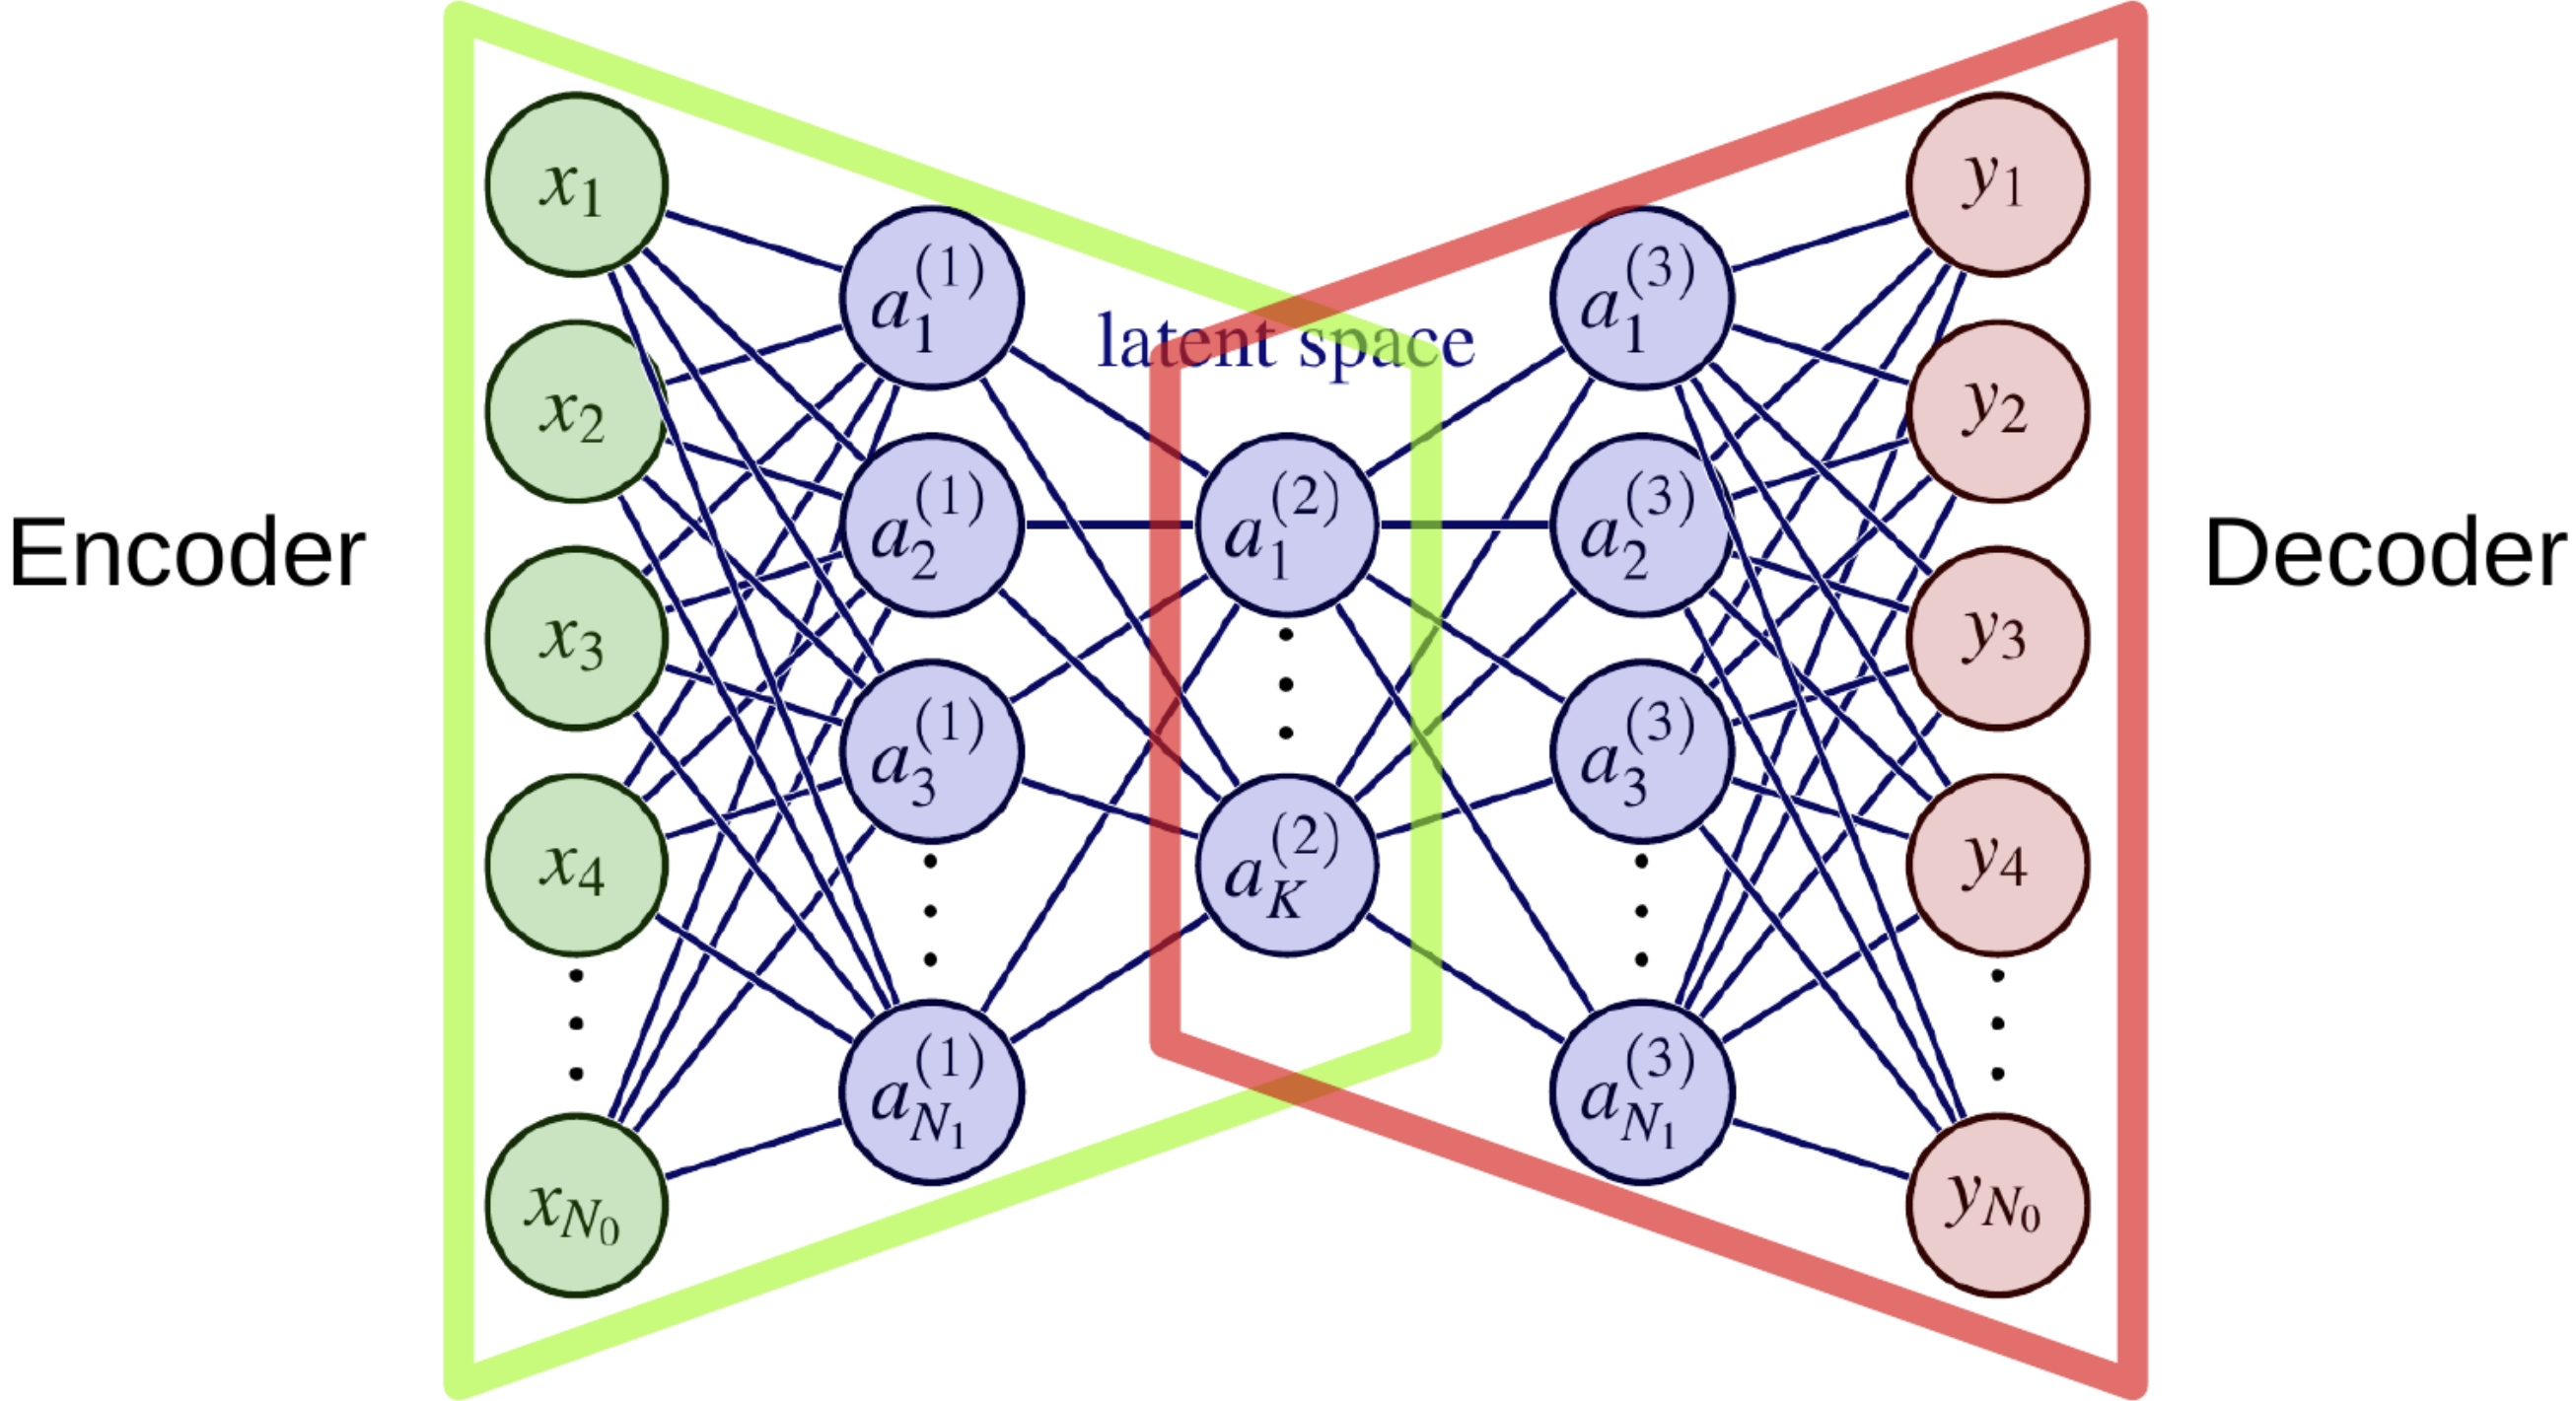
\includegraphics[width=0.45\columnwidth]{figures/Autoencoder.png}
    \vspace{-40pt}
\end{wrapfigure}
\begin{itemize}
    \item \textcolor{green}{Encoder} $F_\theta : \mathbb{R}^{N_0} \to \mathbb{R}^K$
    \item \textcolor{red}{Decoder} $G_{\tilde{\theta}} : \mathbb{R}^K \to \mathbb{R}^{N_0}$
    \item \textbf{Goal:} Minimize \textit{dissimiliarity} function $\ell: \mathbb{R}^{N_0} \times \mathbb{R}^{N_0} \mapsto \R_+$: 
\end{itemize}
$$
\arg \min_{(\theta, \tilde{\theta})} \frac{1}{m} \sum_{i=1}^m \ell(G_{\tilde{\theta}}(F_\theta(x_i)), x_i)
$$

\begin{itemize}
    \item \textbf{Sparse Auto-encoders (SAEs):} Penalty on latent activations. Encourage sparsity: $\mathcal{R}(F_{\theta}(x)) = \lambda |F_{\theta}(x)|_1$.
    \item \textbf{Denoising Auto-encoders (DAEs):} Train on corrupted inputs $\tilde{x} \sim C(\cdot | x)$. Minimize $\ell(x, G_{\hat{\theta}}(F_{\theta}(\tilde{x})))$. 
    \item \textbf{Contractive Auto-encoders (CAEs):} Penalty on input gradient: $\lambda |\nabla_x F_{\theta}(x)|_F^2$. Encourage robust latent representations (i.e., representations that locally do not change much).
\end{itemize}

\textit{\textbf{Example: Categorical Feature Embedding}}

Compress high-dimensional one-hot encoded categorical features (common for insurance datasets) using autoencoders into low-dimensional embeddings; then use these latent representations in the model.


\section{GNNs \& Transformers}

\textbf{Key Idea:} Combine flexibility of NNs with relational structure learning. GNNs leverage \textit{inductive biases} to learn from graph-structured data, capturing relationships between entities.

\subtitle{Graph Neural Networks}

\textbf{Graph Data:} $G=(V,E)$ with Node data: $x_v \in \mathbb{R}^{d_V}$ for $v \in V$; Edge data: $x_e \in \mathbb{R}^{d_E}$ for $e \in E$; and Global data: $u \in \mathbb{R}^{d_U}$.

\textbf{Aggregation functions:} used to aggregate information across all edges
connected to a given node (with varying \#edges).

\begin{subbox}{Graph Net Layer}
    Transforms graphical input data into graphical output data of the same shape.
\begin{enumerate}
    \item \textbf{Edge transform:} $x_e' = \phi^E(x_e, x_v, x_w, u)$ for $e=(v,w)$. \\
    Edge $\rightarrow$ node agg.: $a_w = \rho^{E\to V}(\{x_e': e=(v,w)\})$. \\
    Edge $\rightarrow$ global agg.: $a_E = \rho^{E\to U}(\{x_e': e \in E\})$
    \item \textbf{Node transform:} $x_v' = \phi^V(a_v, x_v, u)$ \\
    Node $\rightarrow$ global agg.: $a_V = \rho^{V\to U}(\{x_v': v \in V\})$
    \item \textbf{Global transform:} $u' = \phi^U(a_E, a_V, u)$
\end{enumerate}
\end{subbox}

$\Rightarrow$ Reason for efficiency of GNNs is that function $\phi^V$ (respectively its parameters) is \textit{shared among all nodes}, and similarly $\phi^E$ is \textit{shared among all edges}.

\subtitle{Self-Attention Layer}

Feedforward NNs $f_K, f_Q, f_V : \mathbb{R}^d \to \mathbb{R}^d$ (\emph{\textbf{K}eys, \textbf{Q}ueries, \textbf{V}alues})
\begin{scriptsize}
\begin{itemize}
    \item \textbf{Edge transformation:}
    \(
    \phi^E(x_{(v,w)}, x_v, x_w) = \left( A_{(v,w)}, \nu_{(v,w)} \right) := \\ \left( \frac{\langle f_Q(x_w), f_K(x_v) \rangle}{\sqrt{d}}, f_V(x_v) \right) \in \mathbb{R}^{d+1}.
    \)
    \item \textbf{Softmax aggr. ($\rho^{E \mapsto V}$):}
    \(
    a_w = \sum_{e \in E_w} \frac{\exp(A_e)}{\sum_{e' \in E_w} \exp(A_{e'})} \nu_e \in \mathbb{R}^d.
    \)
    \item \textbf{Node transformation:}
    \(
    x'_v = \phi^V(a_v, x_v) = f_O(a_v) \in \mathbb{R}^d.
    \)
\end{itemize}
\end{scriptsize}


\subtitle{Transformers}

\textbf{Key Idea:} Stack self-attention layers for seq. data (esp. text).

\begin{itemize}
    \item Input tokens $w_1,...,w_n$ → embeddings in $\mathbb{R}^d$
    \item Learning objective: predict probability distribution over next token $w_{n+1}$ given $w_1,...,w_n$ (conditional prob. forecasting).
    \item Graph: Full $(V\times V)$ or Causal $\{(i,j): i<j\}$ (i.e., masked attention, so  token at position $j$ can only "pay attention to" tokens at positions $i< $j).
    \item Layer: Multi-head attention + Norm + Residuals
    \item Loss: $\ell(p,y)=\sum_{i=1}^K y_i\log(p_i)$
\end{itemize}

\textbf{Training:}
\textbf{(1) Pretrain:} Large-scale unsupervised (e.g., next token); \textbf{(2) Finetune:} Task-specific via full / frozen / PEFT / LoRA $(W \to W + AB, A\in\mathbb{R}^{d\times r}, B\in\mathbb{R}^{r\times k})$ / Soft-prompting.

\end{small}


% OLD Exercises

\section*{Old Exercises / Exams}

\begin{scriptsize}

\subtitle{Exam: HS23}

\exercise{Let LSE: $\mathbb{R} \to \mathbb{R}$ be the Log-Sum-Exp activation function given by
$\text{LSE}(x) = \log\left(e^{ax} + e^x\right)$ for a parameter $0 < a < 1$.

\textbf{(i)} Prove or disprove that LSE is increasing.

\textbf{(ii)} Prove or disprove that LSE is convex.

\textbf{(iii)} Show that $\text{LeakyReLU}(x) \leq \text{LSE}(x) \leq \text{LeakyReLU}(x) + \log(2)$ for all $x \in \mathbb{R}$, where $\text{LeakyReLU}(x) = \max\{ax, x\}$.}

\solution{
\textbf{(i)} The derivative is given by $\frac{(a \exp(ax) + \exp(x))}{\exp(ax) + \exp(x)}$, which is strictly positive. Hence the LSE is strictly increasing.

\textbf{(ii)} The second derivative is $\frac{(a-1)^2 \exp(ax+x)}{(\exp(ax) + \exp(x))^2}$, which is strictly positive. Hence the LSE is strictly convex.

\textbf{(iii)} This follows from:
$\max\{ax, x\} = \log(\max\{\exp(ax), \exp(x)\}) \leq \log(\exp(ax) + \exp(x)) \leq \log(2 \max\{\exp(ax), \exp(x)\}) = \max\{ax, x\} + \log(2).$
}

\exercise{Prove/Disprove that function $(x, y) \mapsto xy$ is convex on $(0,1)^2$.}
\solution{We know that a smooth function is convex if and only if the Hessian is positive semidefinite. However, the Hessian of the given function is 
$\bigl(\begin{smallmatrix} 0 & 1 \\ 1 & 0 \end{smallmatrix}\bigr)$, which has a negative determinant and is thus not positive semidefinite.}


\exercise{Prove/Disprove that the following functions are kernels on $\mathbb{R}^d$:

\textbf{(i)} $k(x, x') = e^{-\langle x, x' \rangle}$, $x, x' \in \mathbb{R}^d$.

\textbf{(ii)} $k(x, x') = \langle x, x' \rangle^2 + \frac{2 \langle x, x' \rangle}{(1 + \|x\|_2)(1 + \|x'\|_2)}$, $x, x' \in \mathbb{R}^d$.}
\solution{
\textbf{(i)} $k$ is not a kernel. Possible valid counterexamples are the following:
\begin{itemize}
    \item For $d = 1$, take $x_1 = 1$ and $x_2 = -2$, then $(k(x_i, x_j))_{i,j=1}^2 = \bigl(\begin{smallmatrix} 1/e & e^2 \\ e^2 & e^{-4} \end{smallmatrix}\bigr)$ has a negative determinant and therefore fails to be positive semi-definite.
    \item For $d = 2$, take $x_1 = (1, 0)$ and $x_2 = (0, 1)$, then $(k(x_i, x_j))_{i,j=1}^2 = \bigl(\begin{smallmatrix} 1/e & 1 \\ 1 & 1/e \end{smallmatrix}\bigr)$ has a negative determinant and therefore fails to be positive semi-definite.
\end{itemize}

\textbf{(ii)} $\langle x, x' \rangle^2$ defines a kernel via the feature map $x \mapsto (\langle x_i, x_j \rangle)_{i,j=1,\dots,d}$. Defining $f(x) := \frac{1}{1 + \|x\|_2}$, we obtain that $f(x)\langle x, x' \rangle f(x') = \frac{\langle x, x' \rangle}{(1+\|x\|_2)(1+\|x'\|_2)}$ defines a kernel function, since for any $x^1, \dots, x^k \in \mathbb{R}^d$ and $\alpha_1, \dots, \alpha_k \in \mathbb{R}$ and $k \in \mathbb{N}$, we have that
\[
\sum_{i=1}^k \sum_{j=1}^k \alpha_i \alpha_j f(x^i) f(x^j) \langle x^i, x^j \rangle = \sum_{i=1}^k \sum_{j=1}^k (\alpha_i f(x^i)) (\alpha_j f(x^j)) \langle x^i, x^j \rangle \geq 0,
\]
where we have used that $\langle x, x' \rangle$ is (clearly) a kernel function. Finally, since for two kernels $k, k'$ and $\lambda > 0$, we also have by the positive semidefinite criteria that $k + \lambda k'$ is a kernel, we obtain the claim by choosing $k(x, x') = \langle x, x' \rangle^2$, $\lambda = 2$ and $k'(x, x') = \frac{\langle x, x' \rangle}{(1+\|x\|_2)(1+\|x'\|_2)}$.}

\exercise{Let $f : [0,1] \to \mathbb{R}$ be a Lipschitz continuous function with Lipschitz constant $K$.

\textbf{(i)} Show that there exists a constant $C > 0$ such that for all $N \in \mathbb{N}$, there exists a shallow ReLU network $f_N : \mathbb{R} \to \mathbb{R}$ with $N$ hidden neurons such that
$\sup_{x \in [0,1]} |f(x) - f_N(x)| \leq \frac{C}{N}$.

\textbf{(ii)} What is the best such constant $C$?

\textbf{(iii)} Show that for every $\epsilon > 0$, there exists a shallow neural network $f_\epsilon : \mathbb{R} \to \mathbb{R}$ with one hidden neuron and tanh-activation function, i.e., a function of the form
$f_\epsilon(x) = a \tanh(bx + c) + d$, for $a, b, c, d \in \mathbb{R}$, such that $\sup_{x \in [-1,1]} |x - f_\epsilon(x)| \leq \epsilon$.}
\solution{
\textbf{(i)} A $K$-Lipschitz $f : [0,1] \to \mathbb{R}$ can be approximated with a piecewise linear function $f_N$ with the same values as $f$ at $t_i = i/N$, for $i = 0, 1, \dots, N$. In turn, $f_N$ can be realized as a shallow ReLU network with $N$ hidden neurons as follows:
$f_N(x) = \sum_{i=1}^N a_i(x - t_{i-1})^+ + b$, by choosing $b = f(t_0)$, $a_1 = N(f(t_1) - f(t_0))$, \color{solutionGray} and $a_i = (f(t_i) - f(t_{i-1}) - 2f(t_{i-1}) + f(t_{i-2}))$ for $i \geq 2$. Obviously, $f_N$ inherits $K$-Lipschitzness from $f$. For every $x \in [0,1]$, $|f(x) - f_N(x)| \leq \frac{K}{N}$. This shows the claim with $C = K$.

\textbf{(ii)} The optimal constant is $C = K/2$. One way to show this is:
For $x \in [t_i, t_{i+1}]$, write $x = (1-z)t_i + zt_{i+1}$ for some $z \in [0,1]$. Then:
$|f_N(x) - f(x)| \leq |(1-z)f(t_i) + zf(t_{i+1}) - f(x)| \leq \frac{K}{2N}$.

\textbf{(iii)} By a second-order Taylor expansion around zero:
$\tanh(x) = x + \frac{1}{2}\tanh''(\xi)x^2$ for some $\xi$ between $0$ and $x$. Setting $x = hu$, we get:
$\sup_{u \in [-1,1]} \left| \frac{\tanh(hu)}{h} - u \right| \leq hC$. Therefore, we can approximate $u \mapsto u$ within accuracy $\epsilon > 0$ by using $h < \epsilon / C$.}

\exercise{Consider a CART that has been fit to training data $(x_i, y_i) \in \mathcal{X} \times \mathcal{Y}, i = 1, \dots, m$, using a value assignment rule of the form
$
y_t \coloneqq \arg\min_{y \in \mathcal{Y}} \sum_{i=1}^m \mathbb{1}_{\{x_i \in P_t\}} \ell(y, y_i),
$
for a partition of the feature space $\mathcal{X} = \bigsqcup_{t \in \mathcal{T}} P_t$ and a loss function $\ell : \mathcal{Y} \times \mathcal{Y} \to \mathbb{R}$. Give an expression of $y_t$ in terms of $(x_1, y_1), \dots, (x_m, y_m)$ in the following two cases:

\textbf{(i)} [2 Points] $\mathcal{Y} = \mathbb{R}$ and $\ell(y, y') = (y - y')^2$.

\textbf{(ii)} [2 Points] $\mathcal{Y} = \{1, \dots, K\}$ and $\ell(y, y') = \mathbb{1}_{y \neq y'}$.}
\solution{
\textbf{(i)} For each $t$, we have $\sum_{i=1}^m \mathbb{1}_{\{x_i \in P_t\}} \ell(y, y_i) = \sum_{x_i \in P_t} (y - y_i)^2$. By strict convexity, the minimizer is the one with derivative zero. Taking the derivative with respect to $y$ and setting it to zero yields $2 \sum_{x_i \in P_t} (y - y_i) = 0$, which gives $y = \sum_{x_i \in P_t} y_i$. Thus:
$
y_t = \frac{1}{|\{i \in \{1, \dots, m\} : x_i \in P_t\}|} \sum_{x_i \in P_t} y_i.
$

\textbf{(ii)} For each $t$, we have $\sum_{i=1}^m \mathbb{1}_{\{x_i \in P_t\}} \ell(y, y_i) = \sum_{x_i \in P_t} \mathbb{1}_{y \neq y_i}$. Minimizers of this function are clearly the same as maximizers of one minus this function, i.e., maximizers of $\sum_{x_i \in P_t} \mathbb{1}_{y = y_i} = |\{i \in \{1, \dots, m\} : x_i \in P_t, y_i = y\}|$. This yields:
$
y_t = \arg\max_{y \in \mathcal{Y}} |\{i \in \{1, \dots, m\} : x_i \in P_t, y_i = y\}|.
$
}

\exercise{Name different types of feature variables.}
\solution{Ddiscrete, Continuous, Categorical.}

\exercise{Name four different hypothesis classes that are used in machine learning.}
\solution{Affine functions, polynomials, splines, trees or decision trees or classification/regression trees or CART, SVM or support vector machines or RKHS functions,
Neural networks, random forest, gradient boosted trees or AdaBoost, graph neural networks, transformers.}

\exercise{Let $A$ be a real $m \times n$ matrix. What is the best approximation of $A$ with an $m \times n$ matrix $B$ of rank at most $k \leq \min\{m, n\}$ with respect to the spectral norm
$
\|A\|_2 \coloneqq \sup_{x \in \mathbb{R}^n, \|x\|_2 = 1} \|Ax\|_2?
$}
\solution{
As seen in class, $v_1 = \arg\max_{x \in \mathbb{R}^n, \|x\|_2 = 1} \|Ax\|_2^2$, where $v_1$ is the (normalized) eigenvector of $A^\top A$ corresponding to the eigenvalue $\sigma_1^2(A)$, where $\sigma_1(A)$ is the largest singular value of $A$. Therefore, for any matrix $A \in \mathbb{R}^{m \times n}$:
$
\|A\|_2 = \|Av_1\|_2 = \sqrt{v_1^\top A^\top A v_1} = \sigma_1(A).
$

Let $U_k \Sigma_k V_k^\top$ be the truncated SVD of $A$ of rank $k$, then:
$
\|A - U_k \Sigma_k V_k^\top\|_2 = \biggl\| \sum_{i=k+1}^n \sigma_i u_i v_i^\top \biggr\|_2 = \sigma_{k+1}(A).
$

We claim that this value is optimal, that is, if $B \in \mathbb{R}^{m \times n}$ is any matrix with $\text{rank}(B) \leq k$, then
$
\|A - B\|_2 = \sigma_1(A - B) \geq \sigma_{k+1}(A).
$

Indeed, Weyl's inequality for singular values implies:
$
\sigma_i(X) + \sigma_j(Y) \geq \sigma_{i+j-1}(X + Y).
$
For $X = A - B$, $Y = B$, and $j = k+1$ and $i = 1$, this yields:
$
\sigma_1(A - B) \geq \sigma_{k+1}(A),
$
where we have used that $\sigma_{k+1}(B) = 0$ because $\text{rank}(B) = k$.}

\subtitle{Problem Set 1}

\exercise{(Overfitting) Let $(x_i, y_i)$, $i = 1, \dots, m$, be a training set of $m$ independent realizations of $(X, Y)$, where $X$ is a $d$-dimensional random vector with continuous distribution and $Y$ a square-integrable random variable.
Consider empirical square loss min. problem:
\(
\min_{f \in H} \frac{1}{m} \sum_{i=1}^m (f(x_i) - y_i)^2,
\)
where $H$ is a given hypothesis class of functions $f: \mathbb{R}^d \to \mathbb{R}$.
Show that if $H$ is the class of all Borel measurable functions $f: \mathbb{R}^d \to \mathbb{R}$, there exists for every $c \geq 0$ a minimizer $f \in H$ of the problem such that $E[(f(X) - Y)^2] \geq c$.}
\solution{
Define $f^*(x) = \begin{cases} y_i & \text{if } x = x_i, \\ z & \text{otherwise}, \end{cases}$ where $z \in \mathbb{R}$ \color{solutionGray} is to be determined. Then $\frac{1}{m} \sum_{i=1}^m (f^*(x_i) - y_i)^2 = 0$.\\
For $X$ with continuous distribution, $P[X \in \{x_1, \dots, x_m\}] = 0$, so $E[(f(X) - Y)^2] = E[(z - Y)^2] = z^2 - 2zE[Y] + E[Y^2]$. Choosing $z$ appropriately can make $E[(f(X) - Y)^2]$ arbitrarily large, satisfying $E[(f(X) - Y)^2] \geq c$.
}

\subtitle{Problem Set 2}

\exercise{Show that for two convex functions $g, h: \mathbb{R}^d \to \mathbb{R}$, $ag + h$ is convex for every constant $a \geq 0$.}
\solution{For all $x, y \in \mathbb{R}^d$ and $\lambda \in (0, 1)$:
\((ag + h)(\lambda x + (1 - \lambda)y) = ag(\lambda x + (1 - \lambda)y) + h(\lambda x + (1 - \lambda)y) \leq \lambda(ag + h)(x) + (1 - \lambda)(ag + h)(y).\)}

\exercise{Let $h: \mathbb{R}^d \to \mathbb{R}$ be convex and $g: \mathbb{R} \to \mathbb{R}$ a non-decreasing convex function. Show that $g \circ h: \mathbb{R}^d \to \mathbb{R}$ is convex.}
\solution{Since $g$ is non-decreasing, $g(a) \leq g(b)$ for $a \leq b$. The convexity of $h$ implies $h(\lambda x + (1 - \lambda)y) \leq \lambda h(x) + (1 - \lambda)h(y)$. Applying $g$, $g(h(\lambda x + (1 - \lambda)y)) \leq g(\lambda h(x) + (1 - \lambda)h(y)) \leq \lambda g(h(x)) + (1 - \lambda)g(h(y)).$}

\exercise{Show that a convex function $h: \mathbb{R}^d \to \mathbb{R}$ satisfies $h\left(\sum_{i=1}^n \lambda_i x_i\right) \leq \sum_{i=1}^n \lambda_i h(x_i)$ for all $n \in \mathbb{N}$, $x_1, \ldots, x_n \in \mathbb{R}^d$, and $\lambda_1, \ldots, \lambda_n \in \mathbb{R}^+$ such that $\sum_{i=1}^n \lambda_i = 1$.}
\solution{Prove by induction: Base case holds for $n = 2$. Assume true for $n \geq 2$. For $x_1, \ldots, x_{n+1} \in \mathbb{R}^d$ and $\lambda_1, \ldots, \lambda_{n+1} \in \mathbb{R}^+$ such that $\sum_{i=1}^{n+1} \lambda_i = 1$, write $h\left(\sum_{i=1}^{n+1} \lambda_i x_i\right) \leq \lambda_1 h(x_1) + (1 - \lambda_1) h\left(\frac{\sum_{i=2}^{n+1} \lambda_i x_i}{1 - \lambda_1}\right) \leq \sum_{i=1}^{n+1} \lambda_i h(x_i).$}

\exercise{Let $h_i: \mathbb{R}^d \to \mathbb{R}$, $i \in I$, be a family of convex functions where $I$ is a non-empty index set. Show that if $h(x) = \sup_{i \in I} h_i(x)$ is finite for all $x \in \mathbb{R}^d$, then $h$ is convex.}
\solution{For $x, y \in \mathbb{R}^d$ and $\lambda \in (0, 1)$:
$h(\lambda x + (1 - \lambda)y) = \sup_{i \in I} h_i(\lambda x + (1 - \lambda)y) \leq \sup_{i \in I} \{\lambda h_i(x) + (1 - \lambda) h_i(y)\} \leq \lambda h(x) + (1 - \lambda) h(y).$}

\exercise{A subgradient of a function $h: \mathbb{R}^d \to \mathbb{R}$ at a point $x \in \mathbb{R}^d$ is a vector $z \in \mathbb{R}^d$ that satisfies $h(y) - h(x) \geq \langle y - x, z \rangle$ for all $y \in \mathbb{R}^d$. The set of all subgradients $\partial h(x)$ of $h$ at $x$ is called the subdifferential of $h$ at $x$. Show that a function $h: \mathbb{R}^d \to \mathbb{R}$ which has a subgradient at every $x \in \mathbb{R}^d$, is convex.}
\solution{If $z_x \in \mathbb{R}^d$ is a subgradient of $h$ at $x$, then $h(y) \geq h(x) + \langle y - x, z_x \rangle$ for all $y \in \mathbb{R}^d$. Thus, $h(y) = \sup_{x \in \mathbb{R}^d} \{h(x) + \langle y - x, z_x \rangle\}$. Since the supremum of affine functions is convex, $h$ is convex.}

\exercise{It can be shown that a convex function $h: \mathbb{R}^d \to \mathbb{R}$ has a subgradient at every $x \in \mathbb{R}^d$. Use this to show that such a function has a max-representation of the form $h(x) = \max_{(u,v) \in S} \{\langle x, u \rangle + v\}$ for $S = \{(u, v) \in \mathbb{R}^d \times \mathbb{R} : h(x) \geq \langle x, u \rangle + v \text{ for all } x \in \mathbb{R}^d\}$.}
\solution{From the definition of $S$, $h(x) \geq \sup_{(u,v) \in S} \{\langle x, u \rangle + v\}$ for all $x \in \mathbb{R}^d$. Conversely, for $x_0 \in \mathbb{R}^d$, let $z \in \partial h(x_0)$ be a subgradient. Then $h(x) \geq \langle x, z \rangle + h(x_0) - \langle x_0, z \rangle$, implying $(z, h(x_0) - \langle x_0, z \rangle) \in S$ and $h(x_0) = \sup_{(u,v) \in S} \{\langle x_0, u \rangle + v\}$.}

\exercise{Show that the set of minimizers of a convex function $h: \mathbb{R}^d \to \mathbb{R}$ is a convex subset of $\mathbb{R}^d$.}
\solution{Let $x, y \in \mathbb{R}^d$ be minimizers of $h$ and $\lambda \in (0, 1)$. Then $h(\lambda x + (1 - \lambda)y) \leq \lambda h(x) + (1 - \lambda) h(y)$. Since $h(x) = h(y)$ is minimal, $h(\lambda x + (1 - \lambda)y) = h(x) = h(y)$.}

\exercise{A function $h: \mathbb{R}^d \to \mathbb{R}$ is strictly convex if $h(\lambda x + (1 - \lambda)y) < \lambda h(x) + (1 - \lambda) h(y)$ for all $\lambda \in (0, 1)$ and $x, y \in \mathbb{R}^d$ such that $x \neq y$. Show that such a function can have at most one minimizer.}
\solution{Assume $x, y \in \mathbb{R}^d$ are two distinct minimizers of $h$. Then $h(x) = h(y)$ and $h\left(\frac{x + y}{2}\right) < \frac{h(x) + h(y)}{2} = h(x) = h(y)$, a contradiction.}

\exercise{Let $g: \mathbb{R} \to \mathbb{R}$ be of the form $g(x) = g(0) + \int_0^x f(y) dy$ for a non-decreasing function $f: \mathbb{R} \to \mathbb{R}$. Show that $g$ is convex and strictly convex if $f$ is strictly increasing.}
\solution{If $f$ is non-decreasing, for $a < b < c$, $\frac{1}{b - a} \int_a^b f(u) du \leq \frac{1}{c - a} \int_a^c f(u) du$, strictly if $f$ is strictly increasing. Hence for $x < y$ and $\lambda \in (0, 1)$:
$\lambda g(x) + (1 - \lambda) g(y) - g(\lambda x + (1 - \lambda)y) = (1 - \lambda) \int_x^y f(u) du - \int_x^{x + \lambda(y-x)} f(u) du \geq 0$, strictly if $f$ is strictly increasing.}

\exercise{Show that a differentiable function $g: \mathbb{R} \to \mathbb{R}$ is convex if $g'$ is non-decreasing and strictly convex if $g'$ is strictly increasing.}
\solution{Follows from the previous exercise.}

\exercise{Show that a twice differentiable function $g: \mathbb{R} \to \mathbb{R}$ is convex if $g''(x) \geq 0$ for all $x \in \mathbb{R}$ and strictly convex if $g''(x) > 0$ for all except countably many $x \in \mathbb{R}$.}
\solution{Follows from the previous exercise since $g'$ is non-decreasing if $g''(x) \geq 0$ and strictly increasing if $g''(x) > 0$ for all except countably many $x$. For functions $h: \mathbb{R}^d \to \mathbb{R}$, the Hessian $\nabla^2 h(x)$ must be positive semidefinite (convex) or positive definite (strictly convex).}

\exercise{Let $\|\cdot\|$ be a norm on $\mathbb{R}^d$ and $g: \mathbb{R}^+ \to \mathbb{R}$ a non-decreasing convex function. Show that $g(\|\cdot\|)$ defines a convex function from $\mathbb{R}^d$ to $\mathbb{R}$.}
\solution{For all $x, y \in \mathbb{R}^d$ and $\lambda \in (0, 1)$, $\|\lambda x + (1 - \lambda)y\| \leq \lambda \|x\| + (1 - \lambda)\|y\|$. Since $g$ is convex and non-decreasing, $g(\|\lambda x + (1 - \lambda)y\|) \leq g(\lambda \|x\| + (1 - \lambda)\|y\|) \leq \lambda g(\|x\|) + (1 - \lambda) g(\|y\|)$.}

\exercise{Decide whether the following functions are convex, strictly convex or non-convex:
\textbf{(a)} $\sin(x)$, \textbf{(b)} $\frac{e^x}{1 + e^x}$, \textbf{(c)} $\log(x)$, \textbf{(d)} $\log(a + e^{bx})$ for constants $a, b > 0$, \textbf{(e)} $\sum_{i=1}^d |x_i|^p$ for $p \geq 1$.}
\solution{
\textbf{(a)} Non-convex. \textbf{(b)} Non-convex. \textbf{(c)} Non-convex (the second derivative is negative, so $\log$ is strictly concave). \textbf{(d)} The second derivative is positive, so $f$ is strictly convex. \textbf{(e)} Convex for $p = 1$ and strictly convex for $p > 1$.
}

\exercise{For given constants $a, b > 0$ and $n \in \mathbb{N}$, find $x_1, \ldots, x_n > 0$ such that $\frac{a^2 + b^2 \sum_{i=1}^n x_i^2}{\sum_{i=1}^n x_i}$ is minimal.}
\solution{The minimizer satisfies $x_1 = \cdots = x_n = \frac{1}{\sqrt{n}} \frac{a}{b}$, and the minimum value is $\frac{2ab}{\sqrt{n}}$.}

\subtitle{Problem Set 3}

\exercise{(Optimal Linear Separation) Consider a data set \((x_i, y_i) \in \mathbb{R}^d \times \{-1, 1\}, i = 1, \ldots, m\), such that not all \(y_i, i = 1, \ldots, m\), are equal and can be linearly separated, meaning there exist \(w \in \mathbb{R}^d, b \in \mathbb{R}\) such that \(\text{sign}(\langle w, x_i \rangle + b) = y_i\) for all \(i = 1, \ldots, m\). Define \(H(w, b) := \{x \in \mathbb{R}^d : \langle w, x \rangle + b = 0\}\), and let \((w_D, b_D) \in \mathbb{R}^d \times \mathbb{R}\) maximize the distance between data and decision hyperplane among hyperplanes with \(\|w_D\|_2 = 1\): \[
(w_D, b_D) = \operatorname*{arg\,max}_{(w,b) \in \mathbb{R}^d \times \mathbb{R}, \|w\|_2=1, \text{sign}(\langle w,x_i \rangle+b)=y_i} \min_{i \in \{1, \ldots, m\}, p \in H(w,b)} \|x_i - p\|_2. \]
Show that \((w_D, b_D) = (w^*_D/\|w^*_D\|, b^*_D/\|w^*_D\|)\), where \((w^*_D, b^*_D)\) is the optimizer of
\[
\min_{(w,b) \in \mathbb{R}^d \times \mathbb{R}} \langle w, w \rangle \quad \text{subject to: } y_i(\langle w, x_i \rangle + b) \geq 1 \text{ for all } i = 1, \ldots, m.
\]
(You may use without proof that both optimization problems have a unique solution.)}
\solution{For any \(i = 1, \ldots, m\), let \(\bar{x}_i = x_i + z_i\) be the projection of \(x_i\) onto \(H(w, b)\). Then \(z_i = \lambda_i w\) for some \(\lambda_i \in \mathbb{R}\), and \(\langle \bar{x}_i, w \rangle + b = 0\) implies \(\lambda_i \|w\|^2_2 = -b - \langle x_i, w \rangle\). Thus, for a feasible \((w, b)\) of the maximization problem and any \(i = 1, \ldots, m\):
$
\min_{p \in H(w,b)} \|x_i - p\|_2 = \|x_i - \bar{x}_i\|_2 = |\lambda_i| \|w\|_2 = |\lambda_i| = |\langle x_i, w \rangle + b| = y_i(\langle x_i, w \rangle + b).
$
Using this equality, any feasible \((w, b)\) with value \(V\) yields a feasible \((w/V, b/V)\) of the minimization problem with value \(1/V^2\). Conversely, any feasible \((\tilde{w}, \tilde{b})\) with value \(\tilde{V}\) yields a feasible \((\tilde{w}/\|\tilde{w}\|, \tilde{b}/\|\tilde{w}\|)\) of the maximization problem with value \(1/\sqrt{\tilde{V}}\). Since these operations are inverses of each other, the optimizers coincide up to normalization.}

\exercise{(Kernel Functions) Prove that the following are kernel functions on \(\mathbb{R}^d\):
\begin{enumerate}[label=(\alph*)]
  \item Linear kernel: \(k(x, x') = \langle x, x' \rangle\).
  \item Squared kernel: \(k(x, x') = \langle x, x' \rangle^2\).
  \item Monomial kernel: \(k(x, x') = \langle x, x' \rangle^p\) for \(p \in \mathbb{N}\).
  \item Sums of kernels: If \(k\) and \(k'\) are kernels, \(k + k'\) is again a kernel.
  \item Scaling: If \(k\) is a kernel and \(\gamma > 0\), \(\gamma k\) is again a kernel.
  \item Polynomial kernel: \(k(x, x') = (\langle x, x' \rangle + \gamma)^p\) for \(p \in \mathbb{N}\) and \(\gamma > 0\).
  \item Scaling with a function: If \(k\) is a kernel and \(f : \mathbb{R}^d \to \mathbb{R}\) is any function, then \(k'(x, x') = f(x)k(x, x')f(x')\) is again a kernel.
  \item Limits of kernels: Let \(k_1, k_2, k_3, \ldots\) be kernels converging pointwise to a function \(k(x, x') = \lim_{m \to \infty} k_m(x, x')\). Then \(k\) is again a kernel.
  \item Exponential kernel: \(k(x, x') = \exp(\gamma \langle x, x' \rangle)\) for \(\gamma > 0\).
  \item Gaussian kernel: \(k(x, x') = \exp(-\gamma \|x - x'\|^2_2)\) for \(\gamma > 0\).
\end{enumerate}}
\solution{\begin{enumerate}[label=(\alph*)]
  \item By definition, the feature map is the identity map.
  \item Feature map \(\Phi(x) = (x_i x_j)_{i,j=1,\ldots,d}\); then \(\langle x, x' \rangle^2 = \sum_{i,j=1}^d x_i x_j x'_i x'_j = \langle \Phi(x), \Phi(x') \rangle\).
  \item Analogous to (b), with feature map \(\Phi(x) = (x_{i_1} x_{i_2} \cdots x_{i_p})_{i_1,\ldots,i_p=1,\ldots,d}\).
  \item From lin. of the psd criterion: \(\sum_{i,j=1,\ldots,n} \alpha_i \alpha_j \big(k(x_i, x_j) + k'(x_i, x_j)\big) = \sum_{i,j=1,\ldots,n} \alpha_i \alpha_j k(x_i, x_j) + \sum_{i,j=1,\ldots,n} \alpha_i \alpha_j k'(x_i, x_j) \geq 0\).
  \item \(\sum_{i,j=1,\ldots,n} \gamma \alpha_i \alpha_j k(x_i, x_j) = \gamma \sum_{i,j=1,\ldots,n} \alpha_i \alpha_j k(x_i, x_j) \geq 0\), for \(\gamma > 0\) (By linearity of psd criteria).
  \item Polynomial kernel: Expanding \((\langle x, x' \rangle + \gamma)^p\) as \(\sum_{q=0}^p \binom{p}{q} \gamma^{p-q} \langle x, x' \rangle^q\), it can be expressed as a weighted sum of monomial kernels, which are psd by (c), (e), and (d).
  \item \(\sum_{i,j} \alpha_i \alpha_j f(x_i)k(x_i, x_j)f(x_j) = \sum_{i,j} (\alpha_i f(x_i))(\alpha_j f(x_j))k(x_i, x_j) \geq 0\) (By the psd criterion).
  \item Finite sums / limits are interchangeable, preserving psd criterion: \\ \(\sum_{i,j=1,..,n} \alpha_i \alpha_j k(x_i, x_j) = \lim_{m \to \infty} \sum_{i,j=1,..,n} \alpha_i \alpha_j k_m(x_i, x_j) \geq 0\).
  \item Since \(k_m(x, x') = \sum_{j=0}^m \frac{\gamma^j}{j!} \langle x, x' \rangle^j\) is a kernel by (c), (e), and (d), the statement follows by (h).
  \item \(k(x, x') = \exp(-\gamma \|x - x'\|_2^2) = \exp(-\gamma \|x\|_2^2) \exp(2\gamma \langle x, x' \rangle) \exp(-\gamma \|x'\|_2^2)\), and thus the statement follows by (i) and (g).
\end{enumerate}}


\subtitle{Problem Set 4}

\exercise{Let $\psi: \mathbb{R} \to \mathbb{R}$ be the logistic function given by
$\psi(x) = \frac{e^x}{e^x + 1} = \frac{1}{1 + e^{-x}}$.
\textbf{(a)} Find constants $a$, $b$ and $c$ such that $a\psi(bx) + c = \tanh(x)$ for all $x \in \mathbb{R}$.
\textbf{(b)} Compute the derivative of $\psi$ and deduce that $\psi$ is strictly increasing.
\textbf{(c)} Is $\psi$ convex?}
\solution{
\textbf{(a)} The equality holds for $a = b = 2$ and $c = -1$. Indeed,
$2\psi(2x) - 1 = 2\frac{e^{2x}}{e^{2x} + 1} - 1 = \frac{e^{2x} - 1}{e^{2x} + 1} = \frac{e^x - e^{-x}}{e^x + e^{-x}} = \tanh(x)$.
\textbf{(b)} One has
$\psi'(x) = \frac{e^x}{e^x + 1} - \frac{e^{2x}}{(e^x + 1)^2} = \frac{e^x}{(e^x + 1)^2} > 0$ for all $x \in \mathbb{R}$.
So $\psi$ is strictly increasing.
\textbf{(c)} No. One has
$\psi''(x) = \frac{e^x}{(e^x + 1)^2} - \frac{2e^{2x}}{(e^x + 1)^3} = \frac{e^x(1-e^x)}{(e^x + 1)^3} < 0$ for $x > 0$.
Therefore, $\psi$ is strictly concave on $(0,\infty)$, and so, cannot be convex.}

\exercise{Show that the one-dimensional identity function $\mathbb{R} \ni x \mapsto x$ can be represented by a shallow ReLU network with two hidden neurons.}
\solution{Denote $x_+ = \max\{0,x\}$. Then $x = x_+ - (-x)_+$, which is the realization function of a shallow ReLU network with two hidden neurons.}

\exercise{This exercise is about showing that for every $\varepsilon > 0$ there exists a neural network $F_\varepsilon$ with ReLU activation function of width $O(\log(1/\varepsilon))$ and depth $O(\log(1/\varepsilon))$ such that
$\sup_{x \in [-1,1]} |F_\varepsilon(x) - x^2| < \varepsilon$.
\textbf{(i)} Consider the hat function $h: [0,1] \to [0,1]$:
$h(x) = \begin{cases} 2x & x \in [0,\frac{1}{2}) \\ 2(1-x) & x \in [\frac{1}{2},1] \end{cases}$
Let $h_n(x) := (h \circ h \circ ... \circ h)(x)$ be the $n$-fold composition of $h$ with itself. Prove that:
$$h_n(x) = \begin{cases} 2^n(x-\frac{2k}{2^n}) & x \in [\frac{2k}{2^n},\frac{2k+1}{2^n}), k=0,1,...,2^{n-1}-1 \\ 2^n(\frac{2k}{2^n}-x) & x \in [\frac{2k-1}{2^n},\frac{2k}{2^n}), k=1,...,2^{n-1} \end{cases}$$
\textbf{(ii)} Let $f_n: [0,1] \to [0,1]$ be the linear interpolation of $f(x)=x^2$ on the grid points $\{\frac{k}{2^n}, k=0,...,2^n\}$. Show that
$\sup_{x \in [0,1]} |x^2 - f_n(x)| \leq \frac{1}{2^{2n+2}}$.
\textbf{(iii)} Prove that $f_n(x) = f_{n-1}(x) - h_n(x)/2^{2n}$.
\textbf{(iv)} Construct the ReLU network mentioned at the beginning of the exercise and remember to extend the approximation of $x \mapsto x^2$ from $[0,1]$ to $[-1,1]$.}
\solution{\textbf{(i)} The proof follows by induction. For $n=1$ we simply verify that $h_1(x) = h(x)$.
Assume now that the claim is proved for $n-1$ and let's try to compute $h_n(x) = h(h_{n-1}(x))$.
First we fix the following notation:
$I_k^{(n)} = [\frac{2k}{2^n},\frac{2k+1}{2^n}], k=0,...,2^{n-1}-1$, $D_k^{(n)} = [\frac{2k-1}{2^n},\frac{2k}{2^n}], k=1,...,2^{n-1}$.
These are just the sets appearing in the definition of $h_n(x)$. For each $n$, these sets are known as dyadic intervals of order $n$ and form a partition of $[0,1]$ into $2^n$ intervals.
To compute $h_n(x) = h(h_{n-1}(x))$, we now notice that $h_{n-1}(x) \in [0,1/2)$ if $x \in I_k^{(n)} \cup D_k^{(n)}$ for $k$ even, while $h_{n-1}(x) \in [1/2,1]$ if $x \in I_k^{(n)} \cup D_k^{(n)}$ for $k$ odd. In particular we can write:
$h_n(x) = h(h_{n-1}(x)) = \begin{cases} 2h_{n-1}(x) & x \in I_{2k}^{(n)} \cup D_{2k}^{(n)}, \text{ for some } k \\ 2(1-h_{n-1}(x)) & x \in I_{2k-1}^{(n)} \cup D_{2k+1}^{(n)}, \text{ for some } k \end{cases}$
Now we notice that $I_k^{(n-1)} = I_{2k}^{(n)} \cup D_{2k+1}^{(n-1)}$ and $D_k^{(n-1)} = I_{2k-1}^{(n)} \cup D_{2k}^{(n)}$, so we can compute $h_n(x)$ on each dyadic interval of order $n$ and obtain:
$h_n(x) = h(h_{n-1}(x)) = \begin{cases} 2^n(x-\frac{2(2k)}{2^n}) & x \in I_{2k}^{(n)}, \text{ for some } k \\ 2^n(\frac{2(2k)}{2^n}-x) & x \in D_{2k}^{(n)}, \text{ for some } k \\ 2^n(\frac{2(2k+1)}{2^n}-x) & x \in D_{2k+1}^{(n)}, \text{ for some } k \\ 2^n(x-\frac{2(2k-1)}{2^n}) & x \in I_{2k-1}^{(n)}, \text{ for some } k \end{cases}$
which can be re-written more compactly as
$$h_n(x) = h(h_{n-1}(x)) = \begin{cases} 2^n(x-\frac{2k}{2^n}) & x \in I_k^{(n)}, \text{ for some } k \\ 2^n(\frac{2k}{2^n}-x) & x \in D_k^{(n)}, \text{ for some } k \end{cases}$$
and we have therefore recovered the expression for $h_n(x)$ we wanted.

\textbf{(ii)} We can bound the error on each dyadic interval as in the proof of Theorem 2:
$\sup_{x \in [\frac{k}{2^n},\frac{k+1}{2^n}]} |f(x)-f_n(x)| \leq \|f^{(2)}\|_{\infty,[0,1]} \frac{(\frac{k+1}{2^n}-\frac{k}{2^n})^2}{2} = 2\frac{(\frac{1}{2^{n+1}})^2}{2} = \frac{1}{2^{2n+2}}$.

\textbf{(iii)} Since $f_n$ is a linear interpolation, it can be expressed in terms of hat functions as follows:
$f_n(x) = \sum_{k=0}^{2^n} (\frac{k}{2^n})^2 h(2^{n-1}(x-\frac{k-1}{2^n}))$
where $h(2^{n-1}(x-\frac{k-1}{2^n})$ is the hat function centered on $k/2^n$ and vanishing on $(-\infty,(k-1)/2^n]$ and $[(k+1)/2^n,+\infty)$.
We verify that $f_{n-1}(x) - f_n(x) = \frac{1}{2^{2n}}h_n(x)$ on $I_k^{(n)}$:
$f_{n-1}(x) - f_n(x) = (\frac{2k}{2^n})^2\frac{1}{2}(1-2^{n-2}(x-\frac{2k-2}{2^n})) + (\frac{2k+2}{2^n})^2\frac{1}{2}(2^{n-2}(x-\frac{2k}{2^n})) - (\frac{2k}{2^n})^2\frac{1}{2}(1-2^{n-1}(x-\frac{2k-1}{2^n})) - (\frac{2k+1}{2^n})^2\frac{1}{2}(2^{n-1}(x-\frac{2k}{2^n})) = \frac{(2k)^2}{2^{2n}}(-2^{n-1}x + k-1) + \frac{(2k+2)^2}{2^{2n}}(2^{n-1}x-k) - \frac{(2k)^2}{2^{2n}}(-2^{n-1}x+2k-1) - \frac{(2k+1)^2}{2^{2n}}(2^nx-2k) = \frac{(2k)^2}{2^{2n}}(2^{n-1}x-k) + \frac{(2^{n-1}x-k)}{2^{2n}}((2k+2)^2-2(2k+1)^2) = \frac{1}{2^{2n}}(2^nx-2k) = h_n(x)$
A similar computation shows the analogous equality on $D_k^{(n)}$.

\textbf{(iv)} From the previous step we see that $f_n$ must be of the following form:
$f_n(x) = f_0(x) + \sum_{k=1}^n (f_k(x)-f_{k-1}(x)) = x - \sum_{k=1}^n \frac{h_k(x)}{2^{2k}}$.
We can approximate $f_n$ using a ReLU network as follows.
First we notice that the identity and the hat function $h$ can both be represented exactly with shallow ReLU networks as $x = \text{ReLU}(x) - \text{ReLU}(-x)$ and $h(x) = 2\text{ReLU}(x) - 4\text{ReLU}(x-1/2) + 2\text{ReLU}(x-1)$.
Since $h_k$ is the $k$-th composition of $h$ with itself, it can be represented exactly by stacking sequentially $k$ ReLU networks representing $h$.
We can now represent $f_n$ by parallelizing the identity network and each $h_k$ (for $k=1,...,n$) \color{solutionGray} in a single ReLU network. Since each $h_k$ has depth $2k$, these subnetworks do not have the same depth, but we can add layers to the shorter ones by composing with the identity until they all have the same length.
By symmetry of $x \mapsto x^2$, we can extend its approximation from inputs in $[0,1]$ to inputs in $[-1,1]$ simply by composing the ReLU network with $|x| = \text{ReLU}(x) + \text{ReLU}(-x)$.
The final ReLU network approximating $f_n(x)$ has therefore width $3n+2$ and depth $2n+2$.
Therefore, to obtain an approximation error $\varepsilon = \frac{1}{2^{2n+2}}$, we need a ReLU network with width and depth $O(\log(1/\varepsilon))$.}

\exercise{Show that a continuous piecewise linear function $f: [0,1] \to \mathbb{R}$ with $N$ breakpoints can be represented by a shallow ReLU network with $N+1$ hidden neurons.}
\solution{Every continuous piecewise linear function $f: [0,1] \to \mathbb{R}$ with breakpoints $0 < t_1 < ... t_N < 1$ can be written as
$a_0x_+ + \sum_{i=1}^N a_i(x-t_i)_+ + b$
for suitable constants $a_0,a_1,...,a_N$ and $b$, and every function of this form can be realized with a shallow ReLU network with $N+1$ hidden neurons.}

\exercise{Let $F_1, F_2 : \mathbb{R}^d \to \mathbb{R}$ be realization functions of two ReLU networks of the same architecture and $\lambda \in (0, 1)$. Show that, in general, the function $\lambda F_1 + (1 - \lambda) F_2$ cannot be realized by a ReLU network of the same architecture (hence, the realization functions of ReLU networks of a given architecture do not form a convex set).}
\solution{The set $H^\text{ReLU}_{1,N,1}$ of shallow ReLU networks with $N$ hidden neurons can realize continuous piecewise linear functions $f : [0, 1] \to \mathbb{R}$ with $N - 1$ breakpoints. However, the convex combination of two such functions can have up to $2N - 2$ breakpoints, requiring a shallow ReLU network with $2N - 1$ hidden neurons.}

\exercise{Let $F_1, F_2 : \mathbb{R}^d \to \mathbb{R}$ be realization functions of two ReLU networks and $\lambda \in (0, 1)$. Show that there exists a ReLU network that can realize the function $\lambda F_1 + (1 - \lambda) F_2$.}
\solution{Assume $F_1$ and $F_2$ are realizations of ReLU networks with architectures $H^\text{ReLU}_{d,M_1,...,M_{K-1},1}$ and $H^\text{ReLU}_{d,N_1,...,N_{L-1},1}$, respectively. Without loss of generality, assume $K \leq L$. Adding identity layers to the first network matches its depth with the second. The two networks are parallelized into $H^\text{ReLU}_{d,M_1+N_1,...,M_{L-1}+N_{L-1},1}$, and the final affine transformation combines $F_1(x)$ and $F_2(x)$ into $\lambda F_1(x) + (1 - \lambda) F_2(x)$.}

\exercise{Show that for a ReLU network and the square loss function, the empirical loss minimization problem is non-convex in the parameters of the network.}
\solution{Consider a shallow ReLU network with one hidden neuron of the form $(ax + b)_+$ for parameters $a, b \in \mathbb{R}$. The empirical loss $\frac{1}{m} \sum_{i=1}^m ((ax_i + b)_+ - y_i)^2$ is generally not convex in $(a, b)$. For example, if $m = 1$, $x_1 = 0$, and $y_1 = 1$, then $(b_+ - 1)^2$ is not convex in $b$.}

\exercise{Show that if $\bigcup_{N \in \mathbb{N}} H^\rho_{(1,N,1)}$ is dense in $C([0,1])$, then $\bigcup_{N \in \mathbb{N}} H^\rho_{(d,N,1)}$ is dense in $C([0,1]^d)$ for all $d \geq 1$.

\textbf{(a)} Show that the space $Q^k_d$ of homogeneous polynomials of degree $k$ on $\mathbb{R}^d$ is equal to the linear span of functions of the form $(a^T x)^k$ for $a \in \mathbb{R}^d$.

\textbf{(b)} Show that the space $P^k_d$ of polynomials of degree $\leq k$ on $\mathbb{R}^d$ is equal to the linear span of functions of the form $p(a^T x)$ for $p \in P^k_1$ and $a \in \mathbb{R}^d$.

\textbf{(c)} Prove that the linear span of functions of the form $f(a^T x)$ for $f \in C(\mathbb{R})$ and $a \in \mathbb{R}^d$ is dense in $C([0,1]^d)$.

\textbf{(d)} Prove that if $\bigcup_{N \in \mathbb{N}} H^\rho_{(1,N,1)}$ is dense in $C([0,1])$, then $\bigcup_{N \in \mathbb{N}} H^\rho_{(d,N,1)}$ is dense in $C([0,1]^d)$.}
\solution{
\textbf{(a)} The linear span $A^k_d$ of functions of the form $(a^T x)^k$ for $a \in \mathbb{R}^d$ is contained in $Q^k_d$. Assume there exists a polynomial in $Q^k_d \setminus A^k_d$. Then, there exists a non-zero linear functional $\phi: Q^k_d \to \mathbb{R}$ that vanishes on $A^k_d$. Using the multinomial theorem, $\phi((a^T x)^k) = 0$ implies $\phi$ must vanish on all monomials $\prod_{i=1}^d x_i^{k_i}$ of degree $k$, leading to $\phi = 0$, a contradiction.

\textbf{(b)} The claim follows from (a), as any polynomial $p \in P^k_d$ can be decomposed as $p(x) = \sum_{j=0}^k p_j(x)$, where $p_j \in Q^j_d$, and each $p_j$ can be written in terms of $(a^T x)^j$ for $a \in \mathbb{R}^d$.

\textbf{(c)} By (b), $P^k_d = \text{span}\{p(a^T x): p \in P^k_1, a \in \mathbb{R}^d\} \subseteq \text{span}\{f(a^T x): f \in C(\mathbb{R}), a \in \mathbb{R}^d\}$. Since $\bigcup_{k \geq 1} P^k_d$ is dense in $C([0,1]^d)$ by Stone-Weierstrass, the claim follows.

\textbf{(d)} \color{solutionGray} By (c), the linear span of $\{f(a^T x): f \in C(\mathbb{R}), a \in \mathbb{R}^d\}$ is dense in $C([0,1]^d)$. If $\bigcup_{N \in \mathbb{N}} H^\rho_{(1,N,1)}$ is dense in $C([0,1])$, then any $f(a^T x)$ can be approximated by functions in $\bigcup_{N \in \mathbb{N}} H^\rho_{(1,N,1)}$, which implies $\bigcup_{N \in \mathbb{N}} H^\rho_{(d,N,1)}$ is dense in $C([0,1]^d)$.}


\exercise{Let $\rho: \mathbb{R} \to \mathbb{R}$ be a continuous function and $C_c^\infty(\mathbb{R})$ the set of infinitely differentiable functions with compact support $\varphi: \mathbb{R} \to \mathbb{R}$. The goal of this exercise is to show that if the convolution $\rho \ast \varphi$ is a polynomial for all $\varphi \in C_c^\infty(\mathbb{R})$, then $\rho$ must also be a polynomial.

\textbf{(a)} Show that for all $\varphi \in C_c^\infty(\mathbb{R})$, the convolution $\psi: \mathbb{R} \to \mathbb{R}$ given by
$
\psi(x) = (\rho \ast \varphi)(x) = \int_{\mathbb{R}} \rho(x-y)\varphi(y)dy = \int_{\mathbb{R}} \rho(y)\varphi(x-y)dy, \quad x \in \mathbb{R},
$
is infinitely differentiable with
$
\psi^{(n)}(x) = \int_{\mathbb{R}} \rho(x-y)\varphi^{(n)}(y)dy = \int_{\mathbb{R}} \rho(y)\varphi^{(n)}(x-y)dy, \quad x \in \mathbb{R}, n \in \mathbb{N}.
$

\textbf{(b)} Denote by $C_c^\infty([-1,1])$ the set of $C_c^\infty(\mathbb{R})$-functions with support in $[-1,1]$. Show that the metric
$
d(\varphi_1, \varphi_2) = \sum_{n \geq 0} 2^{-n} \frac{\|\varphi_1^{(n)} - \varphi_2^{(n)}\|_\infty}{1 + \|\varphi_1^{(n)} - \varphi_2^{(n)}\|_\infty}
$
turns $C_c^\infty([-1,1])$ into a complete metric vector space.

\textbf{(c)} Show that for every $j \in \mathbb{N}_0$,
$
V_j = \{\varphi \in C_c^\infty([-1,1]) : \rho \ast \varphi$ is polynomial of degree at most $ j\}.
$
is a closed subset of $C_c^\infty([-1,1])$.

\textbf{(d)} Show that if $\rho \ast \varphi$ is a polynomial for every $\varphi \in C_c^\infty([-1,1])$, then $\bigcup_{j \geq 0} V_j = C_c^\infty([-1,1])$, and it follows from Baire’s category theorem that there exists a $k$ such that $V_k$ contains a non-empty open set, which, since $V_k$ is a vector space, implies that $V_k = C_c^\infty([-1,1])$.

\textbf{(e)} Show that there exists a sequence $(\varphi_n)_{n \in \mathbb{N}}$ in $C_c^\infty([-1,1])$ such that $\rho \ast \varphi_n$ converges to $\rho$ uniformly on compact intervals. Deduce that if $\rho \ast \varphi$ is a polynomial for all $\varphi \in C_c^\infty(\mathbb{R})$, then $\rho$ is also a polynomial.}
\solution{
\textbf{(a)} Since $\varphi$ is compactly supported and infinitely differentiable, $\psi(x) = \int_\mathbb{R} \rho(x-y)\varphi(y)dy$ is infinitely differentiable. Differentiating under the integral gives $\psi^{(n)}(x) = \int_\mathbb{R} \rho(y)\varphi^{(n)}(x-y)dy$.

\textbf{(b)} Let $(\varphi_i)_{i \in \mathbb{N}}$ be a Cauchy sequence in $C_c^\infty([-1,1])$. Then, $\varphi_i^{(n)}$ converges uniformly to some $\zeta_n \in C([-1,1])$ for each $n \geq 0$. By dominated convergence, $\zeta_n(x) = \zeta_0^{(n)}(x)$, so $\varphi_i \to \zeta_0$ in the metric $d$.

\textbf{(c)} Let $(\varphi_i)_{i \in \mathbb{N}} \subseteq V_j$ converge to $\varphi \in C_c^\infty([-1,1])$. Since $\rho \ast \varphi_i$ is a polynomial of degree $\leq j$, and convolution is continuous, $\rho \ast \varphi$ is also polynomial of degree $\leq j$, so $\varphi \in V_j$.

\textbf{(d)} Assume $\bigcup_{j \geq 0} V_j \neq C_c^\infty([-1,1])$. Then $\bigcap_{j \geq 0} V_j^c$ is dense by Baire’s category theorem, contradicting the assumption that $\rho \ast \varphi$ is polynomial for all $\varphi \in C_c^\infty([-1,1])$. Thus, $\rho \ast \varphi$ being polynomial for all $\varphi \in C_c^\infty([-1,1])$ implies $\rho$ is a polynomial.

\textbf{(e)} Take $\psi \in C_c^\infty([-1,1])$ with $\int_\mathbb{R} \psi(x)dx = 1$. Define $\varphi_n(x) = n\psi(nx)$. Then $\rho \ast \varphi_n \to \rho$ uniformly on compact intervals. If $\rho \ast \varphi$ is polynomial for all $\varphi$, and $\rho \ast \varphi_n$ converges to $\rho$, $\rho$ must be a polynomial.}

\subtitle{Problem Set 5}

\exercise{For two given matrices, $I$ and $K$, define their convolution as the matrix $I * K$ given by:
$(I * K)_{i,j} := \sum_{m\in\mathbb{Z}}\sum_{n\in\mathbb{Z}} I_{m,n}K_{i-m,j-n}$,
and define their cross-correlation as the matrix $I \boxtimes K$ given by
$(I \boxtimes K)_{i,j} := \sum_{m\in\mathbb{Z}}\sum_{n\in\mathbb{Z}} I_{m+i-1,n+j-1}K_{m,n}$.
Show that if $K \in \mathbb{R}^{m_1\times m_2}$, then $(I \boxtimes K)_{i,j} = (I * \tilde{K})_{i,j}$, where $\tilde{K}$ is obtained by flipping rows and columns of $K$ and shifting its indices by $(i,j) \to (i-m_1,j-m_2)$.}
\solution{The operation of flipping rows and columns corresponds to:
$(i,j) \mapsto (m_1-i+1,m_2-j+1)$,
while shifting the indices by $(m_1,m_2)$ corresponds to
$(i,j) \to (i-m_1,j-m_2)$.
Composing these two index transformations we obtain that $\tilde{K}_{i,j} = K_{1-i,1-j}$. We can now prove:
$(I * \tilde{K})_{i,j} = \sum_{m\in\mathbb{Z}}\sum_{n\in\mathbb{Z}} I_{m,n}\tilde{K}_{i-m,j-n} = \sum_{m\in\mathbb{Z}}\sum_{n\in\mathbb{Z}} I_{m,n}K_{m-i+1,n-j+1} = \\ \sum_{m\in\mathbb{Z}}\sum_{n\in\mathbb{Z}} I_{m+i-1,n+j-1}K_{m,n} = (I \boxtimes K)_{i,j}$}

\exercise{For an integer vector $(k_1,k_2) \in \mathbb{Z}^2$, define the translation operator $\tau_{(k_1,k_2)}$ as the operator that acts on matrices $M \in \mathbb{R}^{m_1\times m_2}$ as $(\tau_{(k_1,k_2)}(M))_{i,j} = M_{i+k_1,j+k_2}$.
Show that $(I * K)$ is translation equivariant, i.e. $\tau_{(k_1,k_2)}(I * K) = (\tau_{(k_1,k_2)}I) * K$, for all $(k_1,k_2) \in \mathbb{Z}^2$.}
\solution{$(\tau_{(k_1,k_2)}(I * K))_{i,j} = \sum_{m\in\mathbb{Z}}\sum_{n\in\mathbb{Z}} I_{m,n}K_{i+k_1-m,j+k_2-n}$ (definition of matrix convolution and $\tau_{(k_1,k_2)}$)
$= \sum_{m\in\mathbb{Z}}\sum_{n\in\mathbb{Z}} I_{m+k_1,n+k_2}K_{i-m,j-n}$ \color{solutionGray} ($(m,n) \mapsto (m-k_1,n-k_2)$)
$= \sum_{m\in\mathbb{Z}}\sum_{n\in\mathbb{Z}} (\tau_{(k_1,k_2)}I)_{m,n}K_{i-m,j-n}$ (definition of $\tau_{(k_1,k_2)}$)
$= ((\tau_{(k_1,k_2)}I) * K)_{i,j}$ (definition of matrix convolution)}

\exercise{A matrix-valued function $K : X \times X \to \mathbb{R}^{n\times n}$ is a matrix-valued kernel if:
i) $K(x,x') = K(x',x)^T$, for all $x,x' \in X$,
ii) for any $m \in \mathbb{N}$, $x_1,\ldots,x_m \in X$ and $y_1,\ldots,y_m \in \mathbb{R}^n$ we have
$\sum_{i=1}^m\sum_{j=1}^m y_i^T K(x_i,x_j)y_j \geq 0$.
Check that the Neural Tangent Kernel of a neural network $F_\theta : \mathbb{R}^{N_0} \to \mathbb{R}^{N_L}$ defined as:
$K(x,x';\theta) = D_\theta F_\theta(x) \cdot D_\theta F_\theta(x')^T$, for all $x,x' \in \mathbb{R}^{N_0}$,
is indeed an $\mathbb{R}^{N_L} \times \mathbb{R}^{N_L}$-valued kernel for each $\theta$.}
\solution{We check properties listed in the definition of matrix-valued kernels:
i) $K(x,x') = K(x',x)^T$, for all $x,x' \in \mathbb{R}^{N_0}$, because
$(K(x,x';\theta))_{j,k} = \sum_p D_{\theta_p}F_{\theta,j}(x)\\ D_{\theta_p}F_{\theta,k}(x')
= \sum_p D_{\theta_p}F_{\theta,k}(x')D_{\theta_p}F_{\theta,j}(x)
= (K(x',x;\theta))_{k,j}$.
ii) For any $m \in \mathbb{N}$, $x_1,\ldots,x_m \in \mathbb{R}^{N_0}$ and $y_1,\ldots,y_m \in \mathbb{R}^{N_L}$ we have
$\sum_{i=1}^m\sum_{j=1}^m y_i^T \\ K(x_i,x_j)y_j \geq 0$,
because $\sum_{i=1}^m\sum_{j=1}^m y_i^T K(x_i,x_j)y_j = \sum_{i=1}^m\sum_{j=1}^m\sum_{k=1}^{N_L} \\ \sum_{\ell=1}^{N_L} y_{i,k}\sum_p D_{\theta_p}F_{\theta,k}(x_i)D_{\theta_p}F_{\theta,\ell}(x_j)y_{j,\ell} = \sum_p(\sum_{i=1}^m y_i^T \cdot D_{\theta_p}F_\theta(x_i))^2 \geq 0$}

\exercise{A family of $\mathbb{R}^n$-valued random variables $\{f(x)\}_{x\in X}$ is a vector-valued Gaussian Process (GP) if for all $m \in \mathbb{N}$ and all $x_1,\ldots,x_m \in X$, $f_1(x_1),\ldots,f_n(x_1),f_1(x_2),\ldots,f_n(x_2),\ldots,f_1(x_m),\ldots,f_n(x_m)$ are jointly Gaussian. Every vector-valued GP is fully characterized by:
• a vector-valued function $\mu : X \to \mathbb{R}^n$ (the mean function), and
• a matrix-valued kernel $C : X \times X \to \mathbb{R}^{n\times n}$ (the covariance kernel)
such that $\mathbb{E}[f(x)] = \mu(x)$ and $\text{Cov}(f(x),f(x')) = C(x,x')$, for all $x,x' \in X$. We write $f \sim \text{GP}(\mu,C)$ for a Gaussian Process with mean $\mu$ and covariance kernel $C$.
Let $F_{\theta_0} : \mathbb{R}^{N_0} \to \mathbb{R}^{N_L}$ be a neural network with $L+1$ layers and parameter initialization $\theta_0 \sim \mathcal{N}(0,I_{P\times P})$, where $P$ is the number of parameters. Prove that as $N_1,\ldots,N_{L-1} \to \infty$ the function $F_{\theta_0}$ converges to an $\mathbb{R}^{N_L}$-valued Gaussian process whose coordinates, $F_{\theta_0,k}$, are iid centered Gaussian processes with covariance kernel $\Sigma^{(L)}$ given by the following recursion:
$\Sigma^{(1)}(x,x') = \frac{x^T \cdot x'}{N_0} + \beta^2$, for all $x,x' \in \mathbb{R}^{N_0}$,
$\Sigma^{(L)}(x,x') = \mathbb{E}_{f\sim\text{GP}(0,\Sigma^{(L-1)})}[\rho(f(x))\rho(f(x'))] + \beta^2$, for all $x,x' \in \mathbb{R}^{N_0}$.}
\solution{The proof follows by induction.
For a network with two layers ($L=1$), there's no limit to take. Due to parameter initialization, the coordinate processes $F_{\theta_0,k}(x) = \frac{1}{\sqrt{N_0}}\sum_{j=1}^{N_0} W_{k,j}^{(1)}x + \beta b_k^{(1)}$ are mutually independent. Furthermore, each $F_{\theta_0,k}(x)$ is a Gaussian process with covariance kernel:
$\mathbb{E}[F_{\theta_0,k}(x)F_{\theta_0,k}(x')] = \mathbb{E}[(\sum_{i=1}^{N_0}\frac{1}{\sqrt{N_0}}W_{k,i}^{(1)}x_i + \beta b_k^{(1)})(\sum_{l=1}^{N_0}\frac{1}{\sqrt{N_0}}W_{k,l}^{(1)}x'_l + \beta b_k^{(1)})]
=\sum_{i=1}^{N_0}\sum_{l=1}^{N_0}\frac{1}{N_0}\mathbb{E}[W_{k,i}^{(1)}W_{k,l}^{(1)}]x_ix'_l + \beta^2\mathbb{E}[b_k^{(1)}b_k^{(1)}]
=\sum_{i=1}^{N_0}\sum_{l=1}^{N_0}\frac{1}{N_0}\delta_{i,l}x_ix'_l + \beta^2\mathbb{E}[b_k^{(1)}b_k^{(1)}]
= \frac{x^T \cdot x'}{N_0} + \beta^2$

Now suppose the claim for a network with $L$ layers is proved. Then for a network with $L+1$ layers, we have that the coordinate processes are given by
$F_{\theta_0,k}(x) = \sum_{j=1}^{N_{L-1}}\frac{1}{\sqrt{N_{L-1}}}W_{k,j}^{(L)}\rho(F_{\tilde{\theta}_0,j}^{(L-1)}(x)) + \beta b_k^{(L)}$,
where $F_{\tilde{\theta}_0}^{(L-1)}(\cdot)$ is the output of the first $L$ layers (with parameters $\tilde{\theta}_0$). As $N_1,\ldots,N_{L-2} \to \infty$, by induction the $F_{\tilde{\theta}_0,j}^{(L-1)}$ are iid $\text{GP}(0,\Sigma^{(L-1)})$ and, conditionally on $F_{\tilde{\theta}_0}^{(L-1)}$, also the coordinates $F_{\theta,k}(x)$ are iid Gaussian processes with (conditional) covariance:
$\mathbb{E}[F_{\theta_0,k}(x)F_{\theta_0,k}(x')|F_{\tilde{\theta}_0}^{(L-1)}] = \frac{1}{N_{L-1}}\sum_{\ell=1}^{N_{L-1}}\rho(F_{\tilde{\theta}_0,\ell}^{(L-1)}(x))\rho(F_{\tilde{\theta}_0,\ell}^{(L-1)}(x')) + \beta^2$.
Since the terms \\ $\rho(F_{\tilde{\theta}_0,\ell}^{(L-1)}(x))\rho(F_{\tilde{\theta}_0,\ell}^{(L-1)}(x'))$ are iid random variables, by the law of large numbers the normalized sum converges to their common expectation $\mathbb{E}_{f\sim\text{GP}(0,\Sigma^{(L-1)})}[\rho(f(x))\rho(f(x'))]$ as $N_{L-1} \to \infty$, which gives us the expression in the statement of the theorem.}

\exercise{Let $F_{\theta_0}: \mathbb{R}^{N_0} \to \mathbb{R}^{N_L}$ be a neural network with $L+1$ layers and initialized with $\theta_0 \sim N(0, I_{P\times P})$, where $P$ is the number of parameters. Prove that at initialization we have $K^{(L)}(x,x';\theta_0) \stackrel{P}{\to} \tilde{K}^{(L)}(x,x')I_{N_L\times N_L}$ as $N_1,\ldots,N_{L-1} \to \infty$ where the scalar kernel $\tilde{K}^{(L)}$ is defined recursively as:
$\tilde{K}^{(1)}(x,x') = \Sigma^{(1)}(x,x')$
$\tilde{K}^{(L)}(x,x') = \tilde{K}^{(L-1)}(x,x')\dot{\Sigma}^{(L)}(x,x') + \Sigma^{(L)}(x,x')$
where $\dot{\Sigma}^{(L)}(x,x') = E_{f\sim GP(0,\Sigma^{(L-1)})}[\rho'(f(x))\rho'(f(x'))]$}
\solution{The proof follows by induction. For L=1, the NTK is:
$K^{(1)}_{k,j}(x,x') = \sum_{\theta_p} D_{\theta_p}F_{\theta,k}(x)D_{\theta_p}F_{\theta,j}(x') = (\frac{x^T\cdot x'}{N_0} + \beta^2)\delta_{k,j} = \Sigma^{(1)}(x,x')\delta_{k,j}$

For L+1 layers, split sum over first L layers ($\tilde{\theta}$) and last layer. First L layers contribute:
$\frac{1}{N_{L-1}}\sum_{\tilde{\theta}_p}\sum_{i,l} W^{(L)}_{k,i}\rho'(F^{(L-1)}_{\tilde{\theta},i}(x))D_{\tilde{\theta}_p}F^{(L-1)}_{\tilde{\theta},i}(x) \\ W^{(L)}_{j,l}\rho'(F^{(L-1)}_{\tilde{\theta},l}(x'))D_{\tilde{\theta}_p}F^{(L-1)}_{\tilde{\theta},l}(x')$.
As $N_1,\ldots,N_{L-2} \to \infty$, by induction $\sum_{\tilde{\theta}_p}D_{\tilde{\theta}_p}F^{(L-1)}_{\tilde{\theta},i}(x)D_{\tilde{\theta}_p}F^{(L-1)}_{\tilde{\theta},l}(x') \to \tilde{K}^{(L-1)}(x,x')\delta_{i,l}$.
Let $N_{L-1} \to \infty$ and apply LLN:
$\delta_{k,j}E_{f\sim GP(0,\Sigma^{(L-1)})}[\rho'(f(x))\rho'(f(x'))]\tilde{K}^{(L-1)}(x,x')$.
Last layer contributes $\Sigma^{(L)}(x,x')\delta_{j,k}$}

\exercise{Verify that $F_{\theta_t}(x) = F_{\theta_0}(x) + \sum_{i=1}^m\sum_{j=1}^m\sum_{k=1}^m \tilde{K}^{(L)}(x,x_i)\bar{K}^{-1}_{i,j}(\delta_{j,k} - (e^{-2\bar{K}t/m})_{j,k})(y_k - F_{\theta_0}(x_k))$ is solution of $\partial_t F_{\theta_t}(x) = \\ -\frac{2}{m}\sum_{i=1}^m \tilde{K}^{(L)}(x,x_i)(F_{\theta_t}(x_i) - y_i)$}
\solution{Differentiate w.r.t. t:
$\partial_t F_{\theta_t}(x) = \sum_{i,j,k} \tilde{K}^{(L)}(x,x_i)\bar{K}^{-1}_{i,j}\frac{2}{m}\sum_{\ell} \bar{K}_{j,\ell}(e^{-2\bar{K}t/m})_{\ell,k}(y_k - F_{\theta_0}(x_k))$
$= \\ \sum_{i,\ell,k} \tilde{K}^{(L)}(x,x_i)\frac{2}{m}\delta_{i,\ell}(e^{-2\bar{K}t/m})_{\ell,k}(y_k - F_{\theta_0}(x_k))$
$= \\ -\frac{2}{m}\sum_i \tilde{K}^{(L)}(x,x_i)\sum_k (e^{-2\bar{K}t/m})_{i,k}(F_{\theta_0}(x_k) - y_k)$

Only need to show $\sum_k (e^{-2\bar{K}t/m})_{i,k}(F_{\theta_0}(x_k) - y_k) = F_{\theta_t}(x_i) - y_i$.
This follows from solving matrix ODE: $\partial_t F(t) = AF(t)$ with $F(t) = e^{tA}F(0)$}

\exercise{Given dataset $D=((x_i,y_i), 1\leq i\leq m)$ and RKHS $H$ with kernel $K$, show that minimum-norm interpolator, i.e. solution to $\inf_{f\in H, f(x_i)=y_i} \|f\|_H$ is $f^*(x) = \sum_{i=1}^m\sum_{j=1}^m K(x,x_i)\bar{K}^{-1}_{i,j}y_j$}
\solution{Look in subspace $\tilde{H} = \{\sum_{i=1}^m \alpha_i K(\cdot,x_i), \alpha_i\in\mathbb{R}\}$. Unique interpolator given by: \\
$f^*(x_k) = \sum_i \alpha_i K(x_k,x_i) = y_k \Leftrightarrow \bar{K}\alpha = y \Leftrightarrow \alpha = \bar{K}^{-1}y$

For $f\in H\setminus\tilde{H}$ interpolating dataset, decompose $f=\tilde{f}+\tilde{f}^\perp$. By reproducing property, $\tilde{f}^\perp(x_k)=0$ so $\tilde{f}=f^*$. But $\|f\|_H = \|f^*+\tilde{f}^\perp\|_H = \|f^*\|_H + \|\tilde{f}^\perp\|_H > \|f^*\|_H$}

\exercise{Consider model $Y=X^T\beta + \epsilon$ where $X=(X_1,\ldots,X_p)$ is $\mathbb{R}^p$-valued with covariance $\Sigma$ and $\epsilon\sim N(0,\sigma^2)$ independent of $X$. For dataset $D$ prove bias-variance decomposition:
$E[(\hat{f}_D(X)-f^*(X))^2|A] = \beta^T\Pi\Sigma\Pi\beta + \frac{\sigma^2}{m}Tr(\hat{\Sigma}^\dagger\Sigma)$
where $\hat{\Sigma}=\frac{1}{m}A^TA$ and $\Pi=I_p-\hat{\Sigma}^\dagger\hat{\Sigma}$}
\solution{Decompose into bias and variance:
$E[(\hat{f}_D(X)-f^*(X))^2|A] = E[(X^T E[\hat{\beta}|A]-X^T\beta)^2|A] + E[(X^T\hat{\beta}-X^TE[\hat{\beta}|A])^2|A]$

For bias: $E[\hat{\beta}|A] = \hat{\Sigma}^\dagger\hat{\Sigma}\beta$ so
$B_A = (({\hat{\Sigma}^\dagger\hat{\Sigma}-I_p})\beta)^T\Sigma(({\hat{\Sigma}^\dagger\hat{\Sigma}-I_p})\beta) = \beta^T\Pi\Sigma\Pi\beta$.
For variance: $V_A = Tr(Cov(\hat{\beta}|A)\Sigma)$ where
$Cov(\hat{\beta}|A) = \frac{\sigma^2}{m}\hat{\Sigma}^\dagger$
giving $V_A = \frac{\sigma^2}{m}Tr(\hat{\Sigma}^\dagger\Sigma)$}

\subtitle{Problem Set 6}

\exercise{Prove that for any finite partition $F$ of a feature space $X$ ($\bigcup_{F \in F} F = X$, $|F| < \infty$) and labels $\{y_F \in Y : F \in F\}$, the function $f(x) = \sum_{F \in F} y_F 1_F(x)$ can be realized as a binary tree function.}
\solution{Let us first label the sets in $F$ with $F_1, F_2, \ldots, F_N$, $N = |F|$. A simple way is to grow the tree linearly, so $P() = X$, $P_1 = F_1$, $P_0 = X \setminus F_1$ (and $y_1 = y_{F_1}$), then we only keep growing at the 0 end of the tree: So we continue $P_{(0,1)} = F_2$, $P_{(0,0)} = X \setminus (F_1 \cup F_2)$ (and $y_{(0,1)} = y_{F_2}$), and so on, until $P_{(0,\ldots,0,1)} = F_{N-1}$ (with $y_{(0,\ldots,0,1)} = y_{F_{N-1}}$) and $P_{(0,\ldots,0)} = X \setminus (F_1 \cup F_2 \cup \ldots \cup F_{N-1}) = F_N$ (with $y_{(0,\ldots,0)} = y_{F_N}$).}

\exercise{Assume $X$ is a compact subset of $X_1 \times \cdots \times X_d$ for $X_i = \mathbb{R}$, $i = 1,\ldots,d$, and $Y = \mathbb{R}$. Show that standardized binary trees can approximate any continuous function $f: X \to \mathbb{R}$ arbitrarily well with respect to the sup-norm $\|\cdot\|_\infty$.}
\solution{Note that tree functions can represent arbitrary functions of the form $\sum_{F \in F} y_F 1_F(x)$, where for standardized trees the sets in the partition, $F \in F$, need to be of the form $F = S_1 \times \cdots \times S_d$ for intervals $S_i \subseteq \mathbb{R}$. Take any $f: X \to \mathbb{R}$ continuous and $\varepsilon > 0$. By \color{solutionGray} compactness, $f$ is also uniformly continuous, so we can take $\delta > 0$ such that $|f(x) - f(y)| \leq \varepsilon$ for $\|x - y\|_\infty \leq \delta$. Next, we choose a tree of the form $\sum_{F \in F} y_F 1_F(x)$ with $y_F = f(x_F)$ for some $x_F \in F$, and such that $\|x - y\|_\infty \leq \delta$ for all $x,y \in F$ and all $F \in F$. This yields, for all $x \in X$, and some $\bar{F} \in F$ with $x \in \bar{F}$, $|\sum_{F \in F} y_F 1_F(x) - f(x)| = |y_{\bar{F}} - f(x)| = |f(x_{\bar{F}}) - f(x)| \leq \varepsilon$, and thus the claim.}

\exercise{Consider a classification problem with feature space $X$ and output space $Y = \{1,\ldots,K\}$ for some $K \geq 2$. Show that if $\Phi$ is the entropic impurity $\Phi(q_1,\ldots,q_K) = -\sum_{k=1}^K q_k \log q_k$, the impurity $\bar{I}(T) = \sum_{t\in T} p(t)I(t)$ of the tree equals the empirical loss $\frac{1}{m}\sum_{i=1}^m \ell(f(x_i),q(y_i))$ for $\ell$ given by cross-entropy $\ell(p,q) = -\sum_{k=1}^K q_k \log p_k$, $p,q \in \Delta_K$.}
\solution{As shown in Lemma 7.6, we have $\bar{I}(T) = -\frac{1}{m}\sum_{i=1}^m \log(f(x_i,y_i))$ where the introduced notation and the one from the lecture relate via $f(x_i,y_i) = f_{y_i}(x_i)$. On the other hand, we calculate $\frac{1}{m}\sum_{i=1}^m \ell(f(x_i),q(y_i)) =  -\frac{1}{m}\sum_{i=1}^m \\ \sum_{k=1}^K q_k(y_i) \log(f_k(x_i)) = -\frac{1}{m}\sum_{i=1}^m \log(f_{y_i}(x_i)) = -\frac{1}{m}\sum_{i=1}^m \log(f(x_i,y_i))$}

\exercise{Show that if $\Phi$ is the Gini impurity $\Phi(q_1,\ldots,q_K) = \frac{1}{2}\sum_{k=1}^K q_k(1-q_k)$, the impurity $\bar{I}(T) = \sum_{t\in T} p(t)I(t)$ of the tree equals the empirical loss $\frac{1}{m}\sum_{i=1}^m \ell(f(x_i),q(y_i))$ for $\ell$ given by $\ell(p,q) = \frac{1}{2}\sum_{k=1}^K q_k(1-p_k)$, $p,q \in \Delta_K$.}
\solution{This follows from the direct calculation $\bar{I}(T) = \sum_{t\in T} p(t)I(t) = \frac{1}{m}\sum_{t\in T} m_t \frac{1}{2}\sum_{k=1}^K p(k|t)(1-p(k|t)) = \frac{1}{2m}\sum_{t\in T} m_t \sum_{k=1}^K \\ \frac{|\{i \in \{1,\ldots,m\} : x_i \in P_t, y_i = k\}}{m_t}(1-p(k|t)) = \frac{1}{2m}\sum_{t\in T}\sum_{k=1}^K \sum_{i=1}^m 1_{x_i \in P_t} \\  1_{y_i=k}(1-f_k(x_i)) = \frac{1}{m}\sum_{i=1}^m \frac{1}{2}\sum_{k=1}^K q_k(y_i)(1-f_k(x_i))\sum_{t\in T} 1_{x_i \in P_t} = \frac{1}{m}\sum_{i=1}^m \ell(f(x_i),q(y_i))$}

\exercise{Consider a tree growing algorithm for K-fold classification based on an impurity function $I: \Delta_K \to \mathbb{R}_+$. Which conditions does $I$ ideally satisfy? Do the entropic and Gini impurity functions satisfy these conditions?}
\solution{Desirable properties:
1. Continuity: Both functions (entropic and Gini) are continuous
2. Convexity/concavity properties: Both functions are concave
3. Differentiability: Both functions are differentiable, though the derivative of the entropic impurity is not bounded (near 0)
4. The functionals should be minimized at Dirac measures: Both satisfy this by their concavity properties
5. Functions should be maximized at the uniform distribution: Both functionals satisfy this property, again by concavity.}

\exercise{Consider feature and output variables $X: \Omega \to X$ and $Y: \Omega \to Y = \{-1,1\}$ defined on a probability space $(\Omega,F,P)$. What is the theoretically best predictor for the expected exponential loss among all functions $f: X \to \mathbb{R}$ and the corresponding minimal expected loss $\min_{f: X \to \mathbb{R}} E[\exp(-f(X)Y)]$?}
\solution{For a solution to exist, we need that $Y$ takes both positive and negative values almost surely. Notice that: $E[\exp(-f(X)Y) | X] = P(Y=1|X)e^{-f(X)} + P(Y=-1|X)e^{f(X)}$. Deriving with respect to $f(X)$ yields: $\frac{\partial}{\partial f(X)} E[\exp(-f(X)Y) | X] = -P(Y=1|X)e^{-f(X)} + P(Y=-1|X)e^{f(X)}$. Setting this derivative equal to zero: $f(X) = \frac{1}{2}\log\left(\frac{P(Y=1|X)}{P(Y=-1|X)}\right)$, which gives the optimal value $2E[(P(Y=1|X)P(Y=-1|X))^{1/2}]$.}

\exercise{What is the theoretically best predictor for the expected exponential loss among all functions $f: X \to \{1,-1\}$ and the corresponding minimal expected loss $\min_{f: X \to \{1,-1\}} E[\exp(-f(X)Y)]$?}
\solution{Clearly, $f(X) = 1$ if $P(Y=1|X) \geq 1/2$ and $f(X) = -1$, else. Thus, using the notation $p(X) = P(Y=1|X)$, we get the optimal value $E[e^{-1}\max\{p(X),1-p(X)\} + e\min\{p(X),1-p(X)\}]$.}

\end{scriptsize}



\end{document}